
\documentclass[PhD, copyrightpage]{csuthesis} %draft means that it won't actually render any pictures (graphs) it will just include space for them.
% As soon as you get this to compile, your next step
% should be to remove the draft option, so that your
% figures will show up.  Right now it's there so that
% the document will compile as is, with sample figures.

% If the grad school gives you grief for the smallcaps
% (all caps but capital capitals slightly larger) then
% you can use the "nosmallcaps" option to eliminate
% all smallcaps from the preliminary pages.

% The "copyrightpage" option tells the document class
% to generate a copyright page.  If you don't want a
% copyright page, erase that option.

% Now, change the following fields to match your thesis:
%\title{Barium Tagging in Solid Xenon for the nEXO Neutrinoless Double Beta Decay Experiment}
\title{Imaging of Single Barium Atoms in Solid Xenon for the nEXO Neutrinoless Double Beta Decay Experiment}

\author{Timothy Walton}
\departmentname{Department of Physics}
\gradterm{Fall} %The semester that you are going to turn this in.
% The year will automatically be set to the current year.  If you
% want to modify the year manually, use this command:
%\gradyear{2014}
% But otherwise, ignore that command.
\advisor{William M. Fairbank, Jr.}
%\coadvisor{Test Test} %optional
\committee{Robert Wilson \and Bruce Berger \and Alan Van Orden} %separate committee names with \and
%committee names should not have any honorifics (i.e. NO Dr., PhD, professor, etc.)  Just names.

% you do not need these newcommand lines.
% They are my personal shorthand for derivatives.
\newcommand{\deriv}[2]{\frac{\mathrm{d}#1}{\mathrm{d}#2}}
\newcommand{\dby}[1]{\frac{\mathrm{d}}{\mathrm{d}#1}}
\newcommand{\pd}[2]{\frac{\partial#1}{\partial#2}}
\newcommand{\pby}[1]{\frac{\partial}{\partial#1}}

\usepackage{lipsum}%this package provides nonsense text for testing document layouts.  Not needed for real thesis.
\usepackage{color}
\usepackage{xcolor}
\usepackage{amsmath}
\usepackage{braket}

% a couple useful options that you may wish to uncomment:
% \setcounter{tocdepth}{3} %more depth in table of contents
% \numberwithin{equation}{chapter} %display eqn # as 1.3, not 3
% \renewcommand{\bibname}{References} %change the name of your bibliography
% numberwithin commands for table, figure, and section are 
% already included in the .cls file.  You can search for 
% them and remove them if you want to.

\begin{document}
\frontmatter
%turns the page numbering to roman, and does some other stuff.

\begin{abstract}

\begin{center}\textsc{Imaging Single Barium Atoms in Solid Xenon for Barium Tagging in the nEXO Neutrinoless Double Beta Decay Experiment}\end{center}

\vspace{6mm}

The nEXO experiment will search for neutrinoless double beta decay of the isotope \textsuperscript{136}Xe in a ton-scale liquid xenon time projection chamber, in order to probe the Majorana nature of neutrinos. Detecting the daughter \textsuperscript{136}Ba of double beta decay events, called barium tagging, is a technique under investigation which would provide a veto for a background-free measurement. This would involve detecting a single barium ion from within a macroscopic volume of liquid xenon. One proposed barium tagging method is to trap the barium ion in solid xenon at the end of a cold probe, and then detect it by its fluorescence in the solid xenon.  In this thesis, new studies on the spectroscopy of deposits of Ba and Ba\textsuperscript{+} in solid xenon are presented.  Imaging of barium atoms in solid xenon is demonstrated with sensitivity down to the single atom level.  Achievement of this level of sensitivity is a major step toward barium tagging by this method.

%in the search for this decay
\end{abstract}
%\begin{abstract}
%abztrakt
%\end{abstract}
% note that for amsbook (which is basically the class we are copying), the abstract must be declared before the title.  It prints as part of maketitle.
% personally, I put my abstract definition in a separate file, abs_for_diss.tex, and used \input{abs_for_diss} here.
% The grad school requires an abstract.

\begin{acknowledgements}
Bill, Chris, Adam, Shon, Cesar, Brian, Kendy.

If you want the Leif thing, uncomment it in csuthesis.cls.  It says something like "this dissertation is typeset in ... designed by Leif Anderson.
\end{acknowledgements}
%this is optional.  It must be declared before maketitle, a lot like abstract.  Consider having this in a separate file, like ack.tex, and then using \input{ack}

\maketitle
% maketitle is a huge command in a small package.  It will render the title page, copyright page, acknowledgements, abstract, and probably a bunch of other stuff that I'm forgetting about.  If you choose not to define copyright, acknowledgements, etc, it automatically doesn't render them.

% other optional frontmatter could go somewhere in here.  dedication, biography, etc.  Grad school lists approved frontmatter pages somewhere.
% most frontmatter than I consider silly is not yet automated.  Also most frontmatter doesn't have any explicit style requirements, so I feel justified in ignoring it.

\tableofcontents %don't move this around too much
%\listoftables %optional, but this is the spot it should go
%\listoffigures %optional, but this is the right location for it

\mainmatter %switches page numbering to normal, resets page counter, etc.
% This is the start of the main writing, but there are a couple more
% notes that I think might be helpful, tossed in here and there with
% the format testing stuff.

\chapter{Introduction}

Neutrinos have provided illumination as well as great challenge to physics since their discovery.  They first entered our consciousness through W. Pauli, who proposed in 1930 the existence of a neutral, unobserved particle to explain the apparent violation of energy conservation in beta decay. He admitted that neutrinos (then deemed ``neutrons'' -- what we now know as neutrons had not been discovered yet either) should be difficult to observe experimentally, but also that it seemed unlikely that they would never have been noticed before [ref: Pauli letter, or a following paper?].  As it turns out, they are much more difficult to observe than he predicted; they aren't likely to be noticed without extreme experimental techniques.

A theory formulated in 1933 by E. Fermi for beta decay, including the neutrino, would be the beginnings of weak theory, and the development of the very successful Standard Model of particle physics.  But neutrinos continued to challenge theory with the discovery of non-zero neutrino mass, and they remain at the forefront of our exploration of the universe.

The possibility that neutrinos are Majorana particles makes the search for neutrinoless double beta decay very important for the further development of particle theory.  Majorana formulation can describe the origin of neutrino mass, and possibly explain why the mass is very small via the Seesaw Mechanism [ref].  Observation of neutrinoless double beta decay would simultaneously demonstrate that neutrinos are Majorana particles, as well as give a measurement of the absolute mass itself [ref? this is said later too].

To motivate barium tagging, this chapter outlines the current theory for neutrinos, and then describes the neutrinoless double beta decay experiments EXO-200 and nEXO.

\section{Neutrinos}

Neutrinos are chargeless leptons which only interact via the weak force (and gravity).  There are three known ``flavors'' of neutrinos, each corresponding to one of the three known leptons:  $\nu_{e}$, $\nu_{\mu}$, and $\nu_{\tau}$.  These are the eigenstates in the basis of the weak force, so they are the states in which a neutrino will interact via the weak force.

\subsection{Neutrino Oscillation and Mass}

{\color{red}Neutrinos exhibit mixing between their energy eigenstates and their weak force eigenstates, and these are not the same basis. }  {\color{red}\textbf{not really:}  This means that a flavor eigenstate is not a stationary state} {\color{gray}[the fact is that quark mixing happens, and one theory was that neutrinos would do something similar, and then oscillation is discovered...etc...um...well, they could be a different basis, but apparently they would not oscillate if their masses were all zero. You might want to work through the equations assuming zero mass and see what time-evolving a flavor state does ... could they still have 3 different energy states (i.e., momenta)?]--- }a neutrino which begins as a pure flavor state (as all neutrinos will, coming out of a quantum process involving one of the three leptons) will oscillate into the other two flavors as it evolves in time, i.e. the probability of measuring it to be one of the other two flavors is no longer zero.

{\color{gray}\emph{History:  }The first indications of neutrino oscillation came around 1970 with the Ray Davis Experiment [ref.], which measured the flux (at Earth) of solar electron neutrinos.  The flux measured was quite a bit lower than predicted by solar models, and this became known as the Solar Neutrino Problem.  The discovery of neutrino oscillation in the late 1990s [ref.] solved this problem, as only a fraction of the sun's neutrinos, produced as pure electron neutrinos, would interact as such.}

The very small mass of a neutrino, specifically relative to its momentum, lets one write its Hamiltonian in terms of mass squared differences $\Delta m_{ij}^{2} = m_{i}^{2} - m_{j}^{2}$, where $i$,$j$ = 1,2,3, referring to what we then call mass states.  The mass basis is really the energy basis with the small mass approximation, along with dropping some constant terms in the Hamiltonian (which do not affect time evolution).  Writing the time evolution in terms of mass squared differences means that neutrino oscillation experiments can produce measurements of these differences.  In fact, the discovery of neutrino oscillation was the first (and only, so far) demonstration that neutrinos have a non-zero mass.  Without neutrino mass (particularly without differences between the masses of the mass states), neutrinos would not oscillate.

Neutrino oscillation experiments also provide measurements on the amount of mixing between the flavor basis and the mass basis.  We define the mixing between them by a rotation in terms of three mixing angles, $\theta_{12}$, $\theta_{23}$, and $\theta_{13}$.  Transformation between the flavor and mass bases is done with the following unitary matrix, called the Pontecorvo--Maki-–Nakagawa–-Sakata (PMNS) matrix:

\begin{equation}
\begin{aligned}
U &= \begin{pmatrix}
1 & 0 & 0 \\
0 & c_{23} & s_{23} \\
0 & -s_{23} & c_{23} \end{pmatrix}
\begin{pmatrix}
c_{13} & 0 & s_{13} e^{-i \delta} \\
0 & 1 & 0 \\
-s_{13} e^{i \delta} & 0 & c_{13} \end{pmatrix}
\begin{pmatrix}
c_{12} & s_{12} & 0 \\
-s_{12} & c_{12} & 0 \\
0 & 0 & 1 \end{pmatrix}
\begin{pmatrix}
1 & 0 & 0 \\
0 & e^{i \alpha_{1}/2} & 0 \\
0 & 0 & e^{i \alpha_{2}/2} \end{pmatrix} \\
& = \begin{pmatrix}
c_{12} c_{13} & s_{12} c_{13} & s_{13} e^{-i \delta} \\
-s_{12} c_{23} - c_{12} s_{23} s_{13} e^{i \delta} & c_{12} c_{23} - s_{12} s_{23} s_{13} e^{i \delta} & s_{23} c_{13} \\
s_{12} s_{23} - c_{12} c_{23} s_{13} e^{i \delta} & -c_{12} s_{23} - s_{12} c_{23} s_{13} e^{i \delta} & c_{23} c_{13} \end{pmatrix}
\begin{pmatrix}
1 & 0 & 0 \\
0 & e^{i \alpha_{1}/2} & 0 \\
0 & 0 & e^{i \alpha_{2}/2} \end{pmatrix}
\end{aligned}
\label{eqn:umatrix}
\end{equation}

\noindent
where $c_{ij} = \cos \theta_{ij}$ and $s_{ij} = \sin \theta_{ij}$.  $\delta$ is a phase factor related to lepton CP violation, and $\alpha_{i}$ are Majorana phases.

Studying oscillations of neutrinos from different kinds of sources, with different energies and path lengths, can isolate sensitivities to the different parameters {\color{gray}(not really sure if this is the right thing to say)}.  For example, the study of solar neutrinos (neutrinos emanating from nuclear fusion reactions in the core of the sun) provides sensitivity to $\theta_{12}$ and $\Delta m_{12}^{2}$ {\color{gray}(\emph{right? $\theta_{12}$ may not be specifically solar...})}.  Beamline neutrino detectors can be designed for maximum sensitivity to parameters.  The parameters so far measured are as follows in Table  \ref{table:nu_osc_vals}:

\begin{table}[!htbp]
\caption{up to date values with references, and denote ``solar'', ``atmos.'', etc.} %not sure what [Small Table], between \caption and {}, w/ no spaces, does
\label{table:nu_osc_vals}
\begin{tabular}{c|c}
Parameter & Measurement \\
\hline
$\Delta m_{12}^{2}$ & \\
$|\Delta m_{31}^{2}|$ & \\
$\sin^{2} \theta_{12}$ & \\
$\sin^{2} \theta_{23}$ & \\
$\sin^{2} \theta_{13}$ & \\
\end{tabular}
\end{table}

Note that only the absolute value of $\Delta m_{31}^{2}$ is known.  As a consequence, there are two possibilities for the hierarchy of the three neutrino masses.  These are called the Normal and Inverted Hierarchies, as shown in Fig. \ref{fig:numasshier}.

\begin{figure}[H]
        \centering
                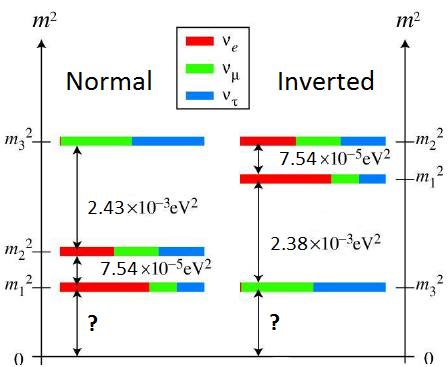
\includegraphics[width=.5\textwidth]{figures/hierarchy_alterred.png}
                \caption{The two possible hierarchies of neutrino masses.  The colors depict the mixing between the mass and flavor bases. {\color{red}\textbf{[ref]}}}
\label{fig:numasshier}
\end{figure}

\noindent
The correct mass hierarchy remains unknown, but next-generation neutrino experiments, possibly including nEXO, will be able to discern this.

Neutrino oscillation demonstrates that neutrinos have non-zero mass, and though oscillation experiments can measure the mass squared differences, we still do not have a measurement of the absolute masses of the three neutrinos.  {\color{gray}\emph{History:  }mention Pauli's first statement of limit near electron mass?  Then maybe say the 0 assumption, which I think came from Fermi's beta decay theory, but if you mention that above, just refer to it here.}

The current upper limits on the mass come from...(KATRIN($\rightarrow \nu_{e}$)?  Cosmology($\rightarrow$ sum)?

Neutrinoless double beta decay experiments like EXO-200 can put upper limits on specifically the Majorana neutrino mass (i.e., upper limits on the neutrino mass if neutrinos are indeed Majorana particles).  As discussed in the next chapter, [EXO-200 and KamLAND (sp?) ZEN (sp?) together provide the strongest Majorana neutrino mass upper limit of [] (IS THAT TRUE?)].

Neutrino oscillation and non-zero neutrino mass are physics beyond the Standard Model (SM) of particle physics, and though much has been discovered through oscillation experiments, there is much yet to learn about neutrinos. Since they are chargeless, they may be Majorana particles, and their small mass could be explained by the See-saw Mechanism [ref]. Majorana particles are their own anti-particle, and this, along with the discovery that neutrinos have mass, allows for a unique test of the Majorana (vs. Dirac) nature of neutrinos: neutrinoless double beta decay.

\subsection{Neutrinoless Double Beta Decay}

Double beta decay is the simultaneous emission of two electrons from a nucleus.  Two-neutrino double beta decay, shown in Fig. \ref{fig:feynman_diags}(left), is allowed by the Standard Model and has been observed in several isotopes which are listed in Table \ref{table:bb_isotopes}.  Similar to beta decay, a neutrino accompanies each electron in this decay, broadening the spectrum of the summed electron energy. This is a second-order process, making it a rare decay, and requiring low backgrounds to measure.

\begin{figure}[H]
        %\centering
        %\begin{subfigure}
                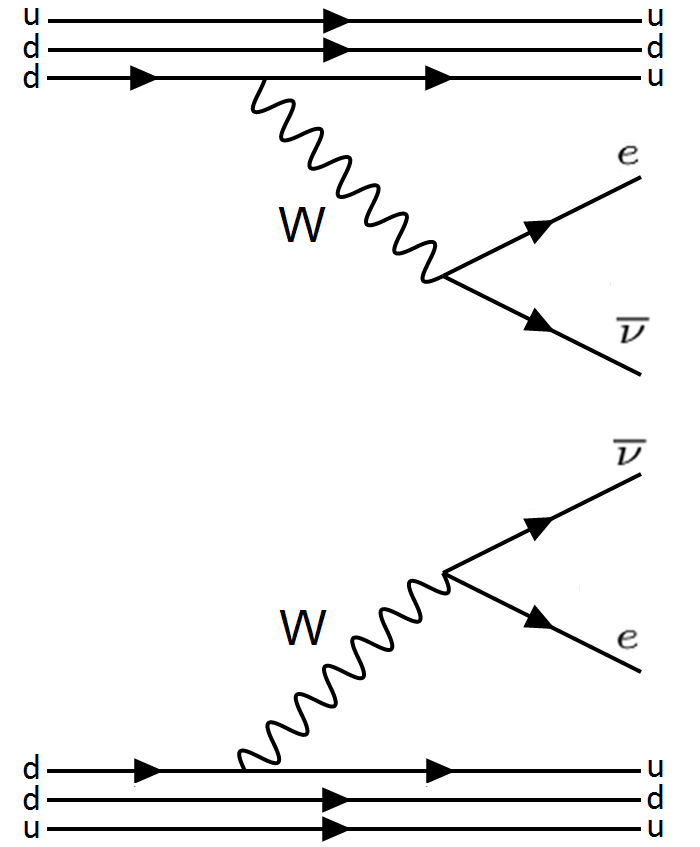
\includegraphics[width=.35\textwidth]{figures/feynman_2nu_quarks.png}
                %\caption{barf}
%        %\end{subfigure}
        %\begin{subfigure}
                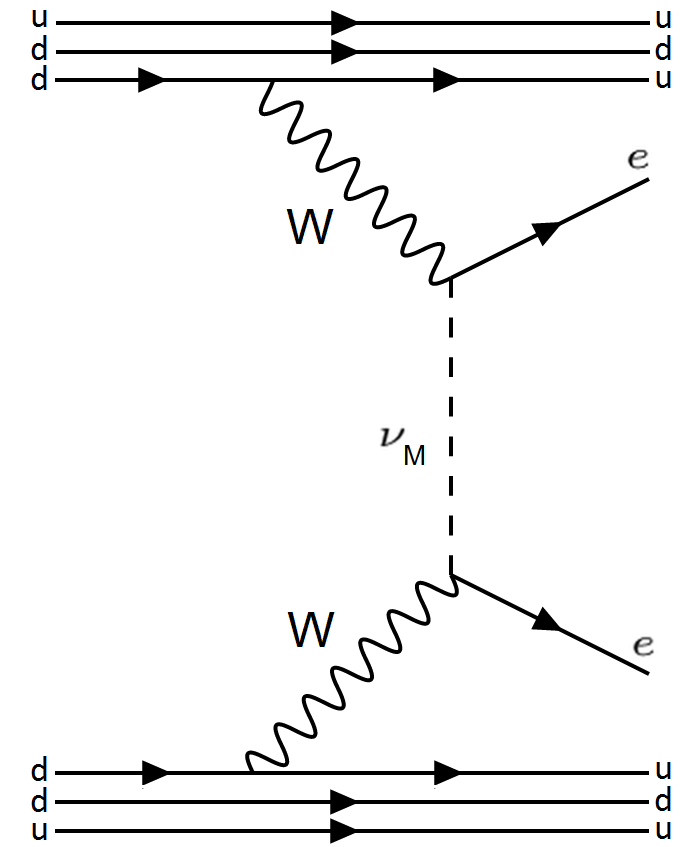
\includegraphics[width=.35\textwidth]{figures/feynman_0nu_quarks.png}
                \caption{Two-neutrino (left) and Neutrinoless (right) double beta decay.}
        %\end{subfigure}
        \label{fig:feynman_diags}
\end{figure}

Neutrinoless double beta decay, shown in Fig. \ref{fig:feynman_diags}(right), is a postulated mode of double beta decay. In this case, the neutrino is exchanged as a virtual particle (which would require that it is a Majorana particle), and there are no neutrinos in the final products. If discovered, not only would neutrinos be determined Majorana particles, but their absolute mass could also be measured in the form of an effective electron neutrino mass, since the rate of neutrinoless double beta decay will depend on the absolute neutrino mass as shown in Eqn. \ref{eqn:rate_vs_mass}:

\begin{equation}
T_{1/2}^{0\nu} = (G^{0\nu}(Q,Z)|M^{0\nu}|^{2}\braket{m_{\nu}}^{2})^{-1}
\label{eqn:rate_vs_mass}
\end{equation}

\noindent
where $T_{1/2}^{0\nu}$ is the $0\nu\beta\beta$ half-life,  $G^{0\nu}$ is a known phase space factor, and $M^{0\nu}$ is a model-dependent nuclear matrix element. The effective electron neutrino mass $\braket{m_{\nu}}$ is the expectation value of the mass for a pure electron neutrino:

\begin{equation}
\braket{m_{\nu}} = \sum\limits_{i} U_{ei}^{2} m_{i}.
\label{eqn:effectivemass}
\end{equation}

The sum of the energies of the emitted electrons in double beta decay will serve as the distinction between the two-neutrino and zero-neutrino modes, shown in Fig. \ref{fig:spectrum_bb}. In the two-neutrino mode, the total decay energy is shared probabilistically between the electrons and the neutrinos (the nucleus recoil energy is negligible), resulting in a broad distribution in the summed electron energy. (Recall the similarly broad electron energy in single beta decay, which ultimately led to discovery of the neutrino involved.) But in the zero-neutrino mode, all of the decay energy is carried away by the two electrons, resulting in only a single allowed value for the summed electron energy -- a peak in the summed electron energy spectrum at the Q-value. 

\begin{figure}[H]
        \centering
                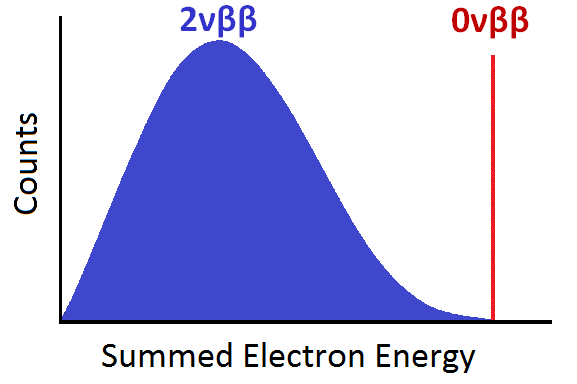
\includegraphics[width=.7\textwidth]{figures/spectrum_bb.png}
                \caption{Conceptual two-neutrino (blue) and zero-neutrino (red) double beta decay spectra.}
\label{fig:spectrum_bb}
\end{figure}

\begin{table}[!htbp]
\caption{$2\nu\beta\beta$ half-lives measured for various isotopes.} %not sure what [Small Table], between \caption and {}, w/ no spaces, does
\label{table:bb_isotopes}
\begin{tabular}{c|c|c}
Isostope & Experiment & $T^{2\nu}_{1/2}$\\
\hline
Xe$_{136}$ & EXO-200 & 2.\\
... & ... & ...\\
\end{tabular}
\end{table}

The rarity of double beta decay (see the very long half lives in Table \ref{table:bb_isotopes}) requires very low backgrounds, especially around the Q-value for the $0\nu\beta\beta$ search. The next sections describe EXO-200 and it's next-generation successor, nEXO.

\section{Enriched Xenon Observatory}

The Enriched Xenon Observatory (EXO) is a set of two experiments, each a LXe time projection chamber (TPC) designed to study the double beta decay of the isotope \textsuperscript{136}Xe, and ultimately to search for the zero-neutrino mode.  There are several advantages to a LXe detector.  Xe is extremely transparent, and scintillates at [around?] [xxx] nm, which is [efficiently collected by [type that the APDs are]] [reference]; so the Xe acts as a detection medium in addition to being the source of the double beta decay [reference? I didn't make up that kind of sentence].  Xe can be continuously purified to maintain large electron lifetimes in the LXe.  Also, the ratio between observed scintillation light and remaining ionized electrons (drifted from the decay site by the TPC's electric field) exhibits a well-known microscopic anti-correlation [ref.], the understanding of which improves the energy resolution of the detector.  Finally, a LXe TPC approach offers the opportunity, [fairly] unique in double beta decay, to reach in and identify, or ``tag'', the daughter Ba\textsuperscript{++} at the site of the double beta decay event, which would provide a background-free identification of neutrinoless double beta decay. Barium tagging is the focus of our group at CSU and is the subject of this thesis.

The following sections decribe the EXO-200 experiment, as well as nEXO, the next-generation tonne-scale LXe TPC which is now in the design stages.  EXO-200 does not have barium tagging implemented, but it is hoped that nEXO will. 

\subsection{EXO-200}

EXO-200 has been operational since April of 20[xx](?).  It is a LXe TPC designed to probe Majorana neutrino masses down to around 100~meV [EXO instrum. paper part I], and is located about half a mile underground in the Waste Isolation Pilot Plant (WIPP) near Carlsbad, NM.  This mine is in a salt basin, which contains lower levels of Uranium and Thorium than a typical mine in rock, making it more ideal for a low-background experiment.  WIPP's main purpose is to permanently store transuranic nuclear waste, which is stored at the other end of the mine and is not an issue for EXO-200.

A schematic of the TPC in the class 100 cleanroom is shown in Fig. \ref{fig:cleanroom}.  Several layers of lead wall surround the copper cryostat, which is filled with hydro-fluoro-ethylwhatever (HFE), a cryogenic fluid which keeps the TPC cooled to LXe temperatures, as well as aids in shielding.  The copper material of the cryostat and TPC is [purified or something?], and is kept as thin as possible to minimize backgrounds.

\begin{figure}[H]
	\centering
	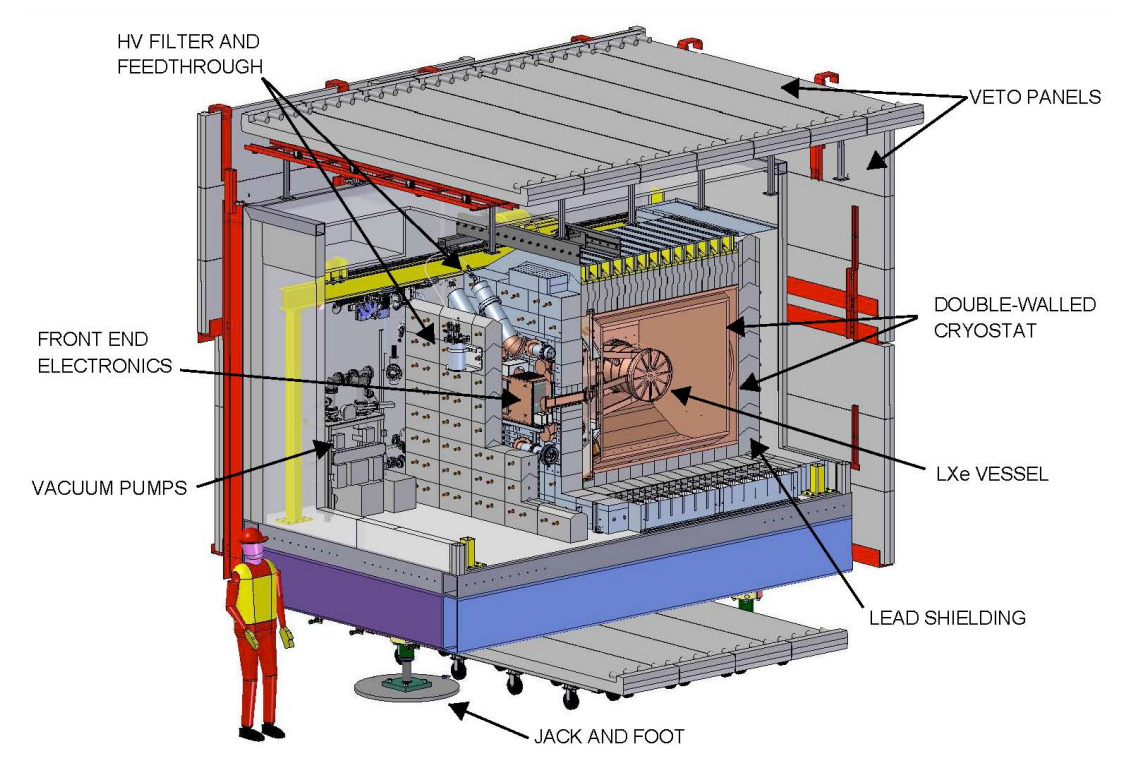
\includegraphics[width=.7\textwidth]{figures/cleanroom.png}
	\caption{Drawing of cleanroom laboratory in the WIPP drift.  \textbf{\color{red} Find better-rez pic.}}
\label{fig:cleanroom}
\end{figure}

Fig. \ref{fig:tpc} shows the EXO-200 detector.  It is actually two face-to-face TPCs which share a cathode.  The detection planes are a combination of ionized charge induction/collection wires and avalanche photodiodes which detect scintillation light.

\begin{figure}[H]
	\centering
	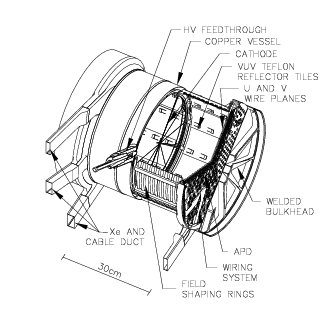
\includegraphics[width=.7\textwidth]{figures/TPC.png}
	\caption{EXO-200 TPC diagram.  [ref $0\nu$ paper or whatev]  {\color{red}Better rez of this too?}}
\label{fig:tpc}
\end{figure}

A photograph of the detection plane is shown in Fig. \ref{fig:tpcphoto}, and a schematic of event detection is shown in Fig. \ref{fig:detectionplane}.  When a double beta decay event occurs in the LXe, the energetic electrons ionize many surrounding Xe atoms.  Some electrons very quickly recombine, emitting scintillation light which is collected by the APDs.  This is part of the energy collection, and also provides a time stamp for the event.  

\begin{figure}[H]
	\centering
	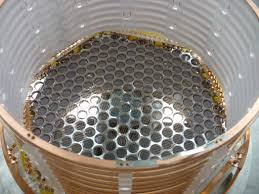
\includegraphics[width=.7\textwidth]{figures/TPCphoto.jpg}
	\caption{View of the detection plane in one of the two EXO-200 TPCs.  [ref $0\nu$ paper or whatev]  {\color{red}I \textbf{know} you have a better rez of this.}}
\label{fig:tpcphoto}
\end{figure}

The cathode is set to 8~kV, providing an electric field of [xxx] V/cm across the 20~cm drift length of each TPC.  Ionized electrons drift from the decay site, first passing the v-wires, which receive an induction signal, and are then collected by the u-wires, which are set at a  {\color{red}60$^\circ$} angle from the v-wires.  The charge collection provides the remainder of the energy collection of the initial decay.

\begin{figure}[H]
	\centering
	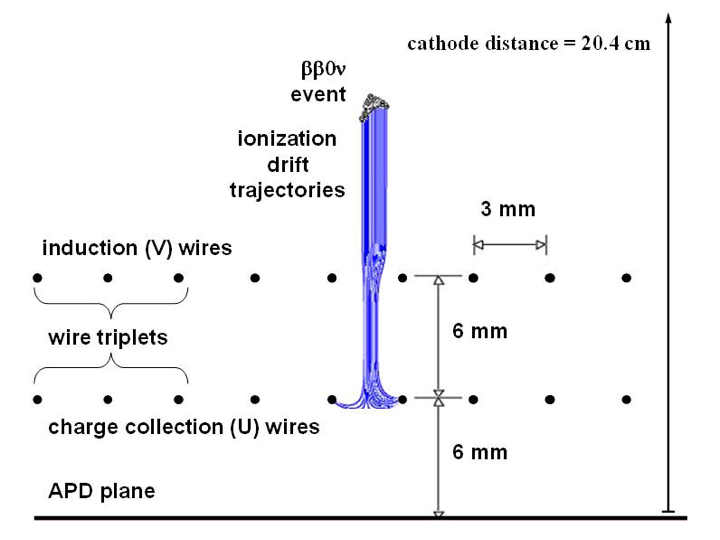
\includegraphics[width=.7\textwidth]{figures/anodecathodedriftcharges.png}
	\caption{EXO-200 event detection.  }
\label{fig:detectionplane}
\end{figure}

Together, the u- and v-wires give an x/y position measurement for the event.  The time between the initial scintillation detection and the charge collection give a z position, and a 3D position can be reconstructed for the event.  

Having a reconstructed 3D event position is important in several ways.  Firstly, position-based corrections on scintillation and charge collection can be applied.  For charge, electronegative impurities in the LXe will absorb the drifting charge, requiring a drift-length (z-position) correction.  High purity levels, measured in terms of electron lifetime, of [???] are maintained in EXO-200, but a small correction of [???] must still be applied [ref].  {\color{red}\textbf{(Is there an x/y purity correction?)}}  For scintillation, a full 3D correction is applied (called the Light Map), as some regions have more efficient light collection by the APDs [ref, maybe for whole paragraph].

A 3D position also allows a fiducial volume to be defined.  The materials of the Teflon walls and cathode/detection planes contain more radioactive background-producing elements.  Radioactive daughters from impurities like radon in the LXe bulk also tend to collect of the cathode [ref], so a stand-off distance of [???] is used as the fiducial cut.

Finally, 3D reconstruction allows the distinction between single-site (SS) and multi-site (MS) events.  A(n?) MS event is one where two spatially separated events occur in the same [???]-$\mu s$ time window.  These are mostly caused by gamma rays interacting in the LXe, which can Compton-scatter several times.  Rejecting MS events strongly separates gamma events from double beta decay events.

Of course, barium tagging will also require a 3D reconstructed position in nEXO.

Calibration of EXO-200 is done using various radioactive sources which can be moved to several positions around the outside of the TPC.  Several different sources span the energy range of interest, but the main source is {\color{red}Th$_{228}$}, which produces gamma rays at [???]~MeV, near the Q-value of Xe$_{136}$ double beta decay where the $0\nu\beta\beta$ peak will be.  Source calibration data also provides a comparison between data and Monet-Carlo simulation, and provides the data for purity measurement and Light Map determination.  Data and Monte-Carlo for Th$_{228}$ are shown in Fig. [ref fig source agreement].

The relationship between scintillation and ionization for a given event in LXe exhibits a well-known anti-correlation.  Applying this to the combination of those signals improves the energy resolution, shown in Fig. [ref fig anticorrelation].  This correction defines a combined energy axis, called the rotated energy.  Energy resolution is important in a $0\nu\beta\beta$ search, as it distinguished those events from $2\nu\beta\beta$ events in the tail of their spectrum.  Resolution of [???] is achieved in [ref $\nu$ paper].

The final data set is fit using a combination of probability distribution functions (PDFs) for $0\nu\beta\beta$, $2\nu\beta\beta$, and all possible backgrounds.  
[data, fitting, measurement and limit]

\subsection{nEXO}

\subsection{Barium Tagging}

lllllllla llllllla lllllla lllllllllllllllla

\noindent
{\color{gray}\textbf{old stupid intro:}

The study of the neutrino has required extremes in experimental technique from the beginning.  Neutrinos were described by W. Pauli, who first proposed their existence to remedy an apparent violation of energy conservation in beta decay, as being [impossible to detect] [ref.].  Rather, it requires a great deal of sensitiviy, ingenuity, and hardship (just "ingenuity and hardship"?  sensitivity may be redundant) to observe them, and it was [] years before they were first observed by [Reines and Cowan] in [], by [] [ref.].  (is "rather, ..." too demoting-sounding?  it is absolutely not meant to be, of course)

Neutrino experiments of greater discovery power have been developed around the world, and command large collaborations of scientists.  ummmmmmmm  this is supposed to kind of allude to barium tagging as an extreme technique

Neutrinoless Double Beta Decay experiments like EXO are a different kind of neutrino experiment, not detecting neutrinos directly, but searching for an effect (neutrinoless double beta decay itself) which would demonstrate the Majorana nature of neutrinos.  A liquid xenon experiment like EXO provides a the challenging opportuniy for another extreme experimental technique, barium tagging, where a single barium ion would be observed at a specific double beta decay site in the volume.  This thesis is part of an exploration of one promising barium tagging technique.  (these things may be saved for the EXO chapter... idk).

From the first formulation of beta decay theory by E. Fermi [ref.], neutrinos have provided an avenue into a world of new physics, and they continue to be such an avenue.  Questions which may be answered by this up and coming generation of neutrino experiments are expected to help explain how the universe came to be this way.

[lead into barium tagging discussion]

section: something like "Can We Do This?", but probably not that at all.

A liquid xenon double beta decay detector allows unique access to the daughters of decays in the liquid volume.  The feasibility of grabbing and detecting a single ion from the volume is what must be determined next.}
\chapter{Theory}
%\label{chap:theory} this doesn't seem to work

%Theory relevant to the spectroscopy and detection of single Ba/Ba\textsuperscript{+} in SXe matrices is discussed.  Spectroscopy of Ba/Ba\textsuperscript{+} is first...

\section{Ba/Ba\textsuperscript{+} Spectroscopy in Vacuum}

The lowest-lying energy levels in vacuum for Ba and Ba\textsuperscript{+} are shown in Fig. \ref{fig:elevs}.  For Ba, the main transition is between the ground $6s^{2}$ $^{1}$S$_{0}$ to the excited $6s6p$ $^{1}$P$_{1}$ state.  Spin{\color{red}(?)}-suppressed transitions between the P state and three metastable D states results in a decay in to a D state after about 350 excitations.  For Ba\textsuperscript{+}, two strong transitions exist between the ground $6s$ $^{2}$S$_{1/2}$ and the $6p$ $^{2}$P$_{1/2}$ and $6p$ $^{2}$P$_{3/2}$ excited states.  Transitions to the two metastable D states are higher than for the atom, resulting in a decay into a D state after about 4 excitations.

\begin{figure}[H]
	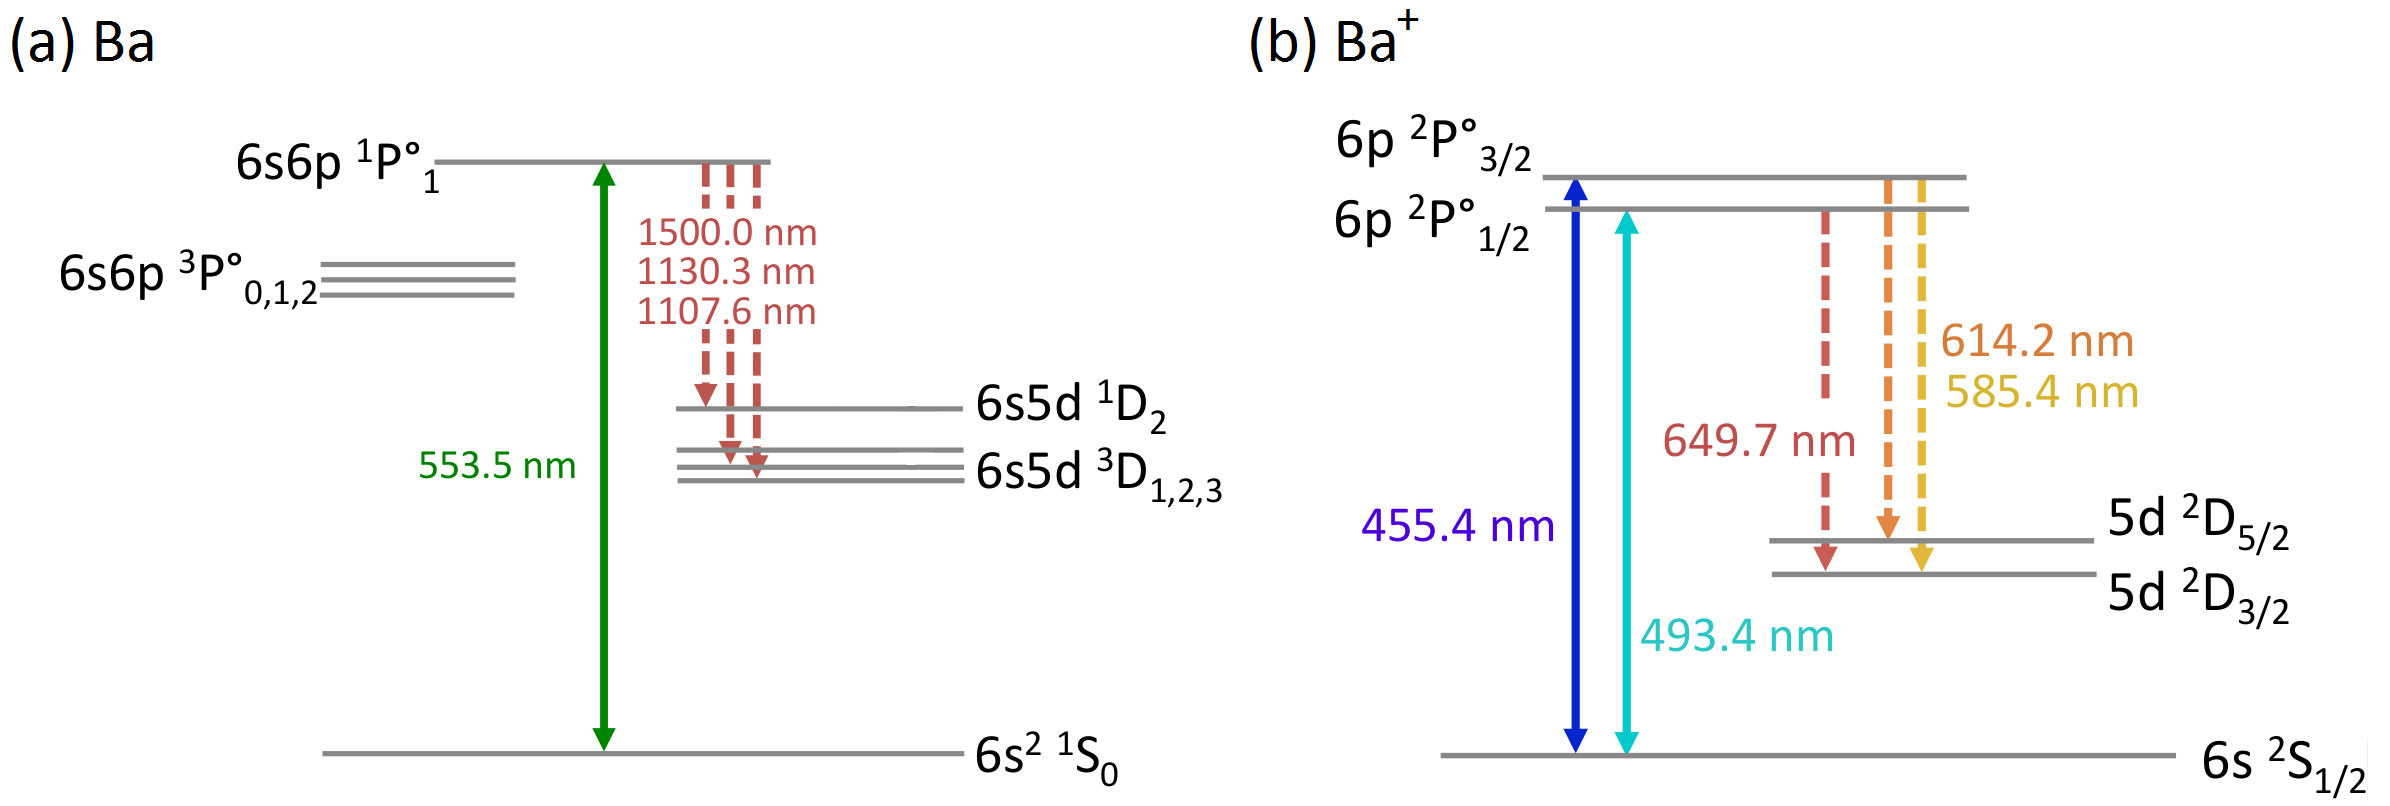
\includegraphics[width=.9\textwidth]{figures/elevs.png}
	\caption{Energy level diagrams for (a) Ba and (b) Ba\textsuperscript{+}}
    \label{fig:elevs}
\end{figure}

These energy levels and their transition rates are well known, and are documented in the NIST Atomic Spectra Database.  Single atom/ion detection by spectroscopy generally requires, in addition to the main excitation laser, lasers to provide transitions out of the metastable D states once the atom/ion decays into one of them.  For the atom, this requires three additional infrared lasers.  Single atom trapping/detection \textbf{\color{red}[do they actually have single-atom in that paper? ... also they did it with a red laser too]} in a magneto-optical trap (MOT) is achieved in \cite{BaMOT}.  Single Ba\textsuperscript{+} observation requires only two lasers if the $^{2}$P$_{1/2}$ excited state is used.  This is demonstrated in [ref something that does this ... is there something?  How about the Carleton group?  I think MOE has a reference to it maybe -- yeah, its [19]].

\section{Matrix Isolation Spectroscopy}

In the solid matrix, the Ba/Ba\textsuperscript{+} spectroscopy is affected by its interaction with neighboring Xe atoms.

\emph{\color{gray}Kind of a main idea is the very different interaction between M and G for the ground vs. excited state.  This leads to Franck-Condon rule and to Jahn-Teller.  Shon doesn't really say that, I don't think.  May just say that it's a van der waal force, w/o writing the force terms, though Crepin doesn't even seem to mention that as important.}

\emph{\color{gray}May be good matrix isolation theory references in Ba Spec... yeah, 1 and 2 i think ... shon's 55, 57, 58 are probably good too and maybe overlapping}

\emph{\color{gray}Does the lead into matrix isolation in Crepin start with just the interaction w/ noble gas?  You could have a section for that like Shon, or just have it within this section.}

The spectroscopy of a species trapped in an inert solid matrix is called matrix isolation spectroscopy, the concept of which was pioneered around 19?? by [that one guy] [ref ... maybe [1] of ba spec].  Though absorption and emission are significantly broadened and shifted, a species can retain properties of its vacuum counterpart, such as quantum numbers.

Studies of some matrix isolation systems have been made.  The most thoroughly studied has been Na(?) in solid matrices of (Ar, Kr, Xe ?)... (Na? Mg?)...[refs]

We are of course interested in the spectroscopy of Ba and/or Ba\textsuperscript{+} in SXe matrices, and this particular system has not been studied until recently.  The first report of the spectroscopy of neutral Ba in SXe, along with candidate fluorescence peaks for Ba\textsuperscript{+} in SXe, was published by our group in [ref ba spec], and conversations following this publication with ???'s group in ??? have confirmed our basic observations of the absorption spectrum of Ba in SXe.  

From here forward I will refer to the host species as Xe and the guest as Ba/Ba\textsuperscript{+}, specific to our system.  The leading interaction between {\color{gray}[put this here if the van der waals is only necessarily the force for Ba in particular]} the Ba/Ba\textsuperscript{+} and a neighboring Xe atom is a {\color{gray}(the)} Van Der Waals (sp?) force, an induced dipole-dipole interaction.  Xe is the most polarizable (sp?) of the noble gases.  

The forms for this force(?) is shown in Eqn. [ref van der ba] for Ba and Eqn. [ref van der ba+] for Ba\textsuperscript{+}.  {\color{gray}Talk about it.}

This binding between the Ba/Ba\textsuperscript{+} and its surrounding Xe atoms results in vibrational modes, and the Franck Condon (sp?) principle applies.  Fig. [ref fig franckcondon] helps illustrate this effect.  In a cold matrix, the system will be in the ground vibrational state before excitation.  The distribution of the wavefunction, even for the ground state alone, overlaps in space in general with more than one of the excited state vibrational modes, resulting in a broadening in energy of the absorption.

Rapid decay occurs to the lowest vibrational mode in the excited state before electronic decay can occur [ref] {\color{red}[is this just for Ba?]}.  Then a similar broadening in emission energy occurs as several overlapping vibrational mode wavefunctions exist in the ground electronic state, and a redshift is also observed as some energy was dissipated into phonons in the crystal in vibrational mode decays.  {\color{blue}\textbf{(How can you get a blueshift?)}}

Shifts and broadening in absorption and emission depend in general on the distribution of Xe atoms around the Ba/Ba\textsuperscript{+}.  The fcc crystal structure of the Xe restricts these environments to discrete number of so-called matrix sites, defined by (a) whether the Ba/Ba\textsuperscript{+} is {\color{red}[intersituational or whatever -- is that still a thing?]}, and (b) the number of vacancies in the Xe matrix surrounding the Ba/Ba\textsuperscript{+}.  Experimental observation of emission peaks from different matrix sites of [Na] in solid noble gases is reported in [ref(s)], with theoretical calculations in [ref(s)] attributing observed peaks to specific vacancy distributions defining the matrix sites (maybe this has been done?).

Energy level transition probabilities can also be affected in a matrix.  Distortions in electron wavefunction shapes by asymmetric matrix sites can affect radiative transitions by altering parity [ref].  If electronic potential energy curves cross each other, nonradiative transitions can also become allowed for otherwise forbidden transitions [ref].  {\color{red}(Is a phonon emission called a nonradiative transition / does this actually happen?)}

\emph{Jahn-Teller?}

The detectability of a single atom/ion can depend greatly on altered transition rates.  For example, in the Ba atom, matrix-allowed decay of the $^{1}$P$_{1}$ to the $^{3}$P states could be much stronger than the main transition back to ground, which would suppress fluorescence and make single-atom detection impossible.  But the matrix could also help by strengthening decays from the D states back to ground, eliminating any need for re-pump lasers to keep the transition cycle going.  

\subsection{6-level System}

Neutral Ba in vacuum is only a 5-level system.  However, solving a 6-level system is helpful in modeling matrix-isolated Ba where interactions could allow a transition into a \textsuperscript{3}P state.

\section{shon had a flu eff section}
%this is now a subsection of intro
\chapter{Experimental}

%\emph{\color{gray}Probably need to mention CCD digitaztion pedestal and noise, and dark counts which are zero when cold -- did you do that?.}

%\noindent
%\emph{

This chapter describes the apparatus at Colorado State University which was used for producing and observing  deposits of Ba/Ba\textsuperscript{+} in SXe.  The main barium source, a Ba\textsuperscript{+} ion beam, is first described, as well as a neutral Ba getter source.  The co-deposit of Ba/Ba\textsuperscript{+} with Xe gas onto a cold sapphire window, subsequent laser excitation, and finally the collection optics for the fluorescence are described.

\section{Ion Beam}

The ion beam system is shown in Fig. \ref{fig:ionbeam}.  This is a clean source of Ba\textsuperscript{+} which can do a very wide range of deposit sizes, from billions of ions in a focused laser region all the way down to the single-ion level and below.
%(may only want to say that if we have those scans)

\begin{figure} %[H]
        \centering
                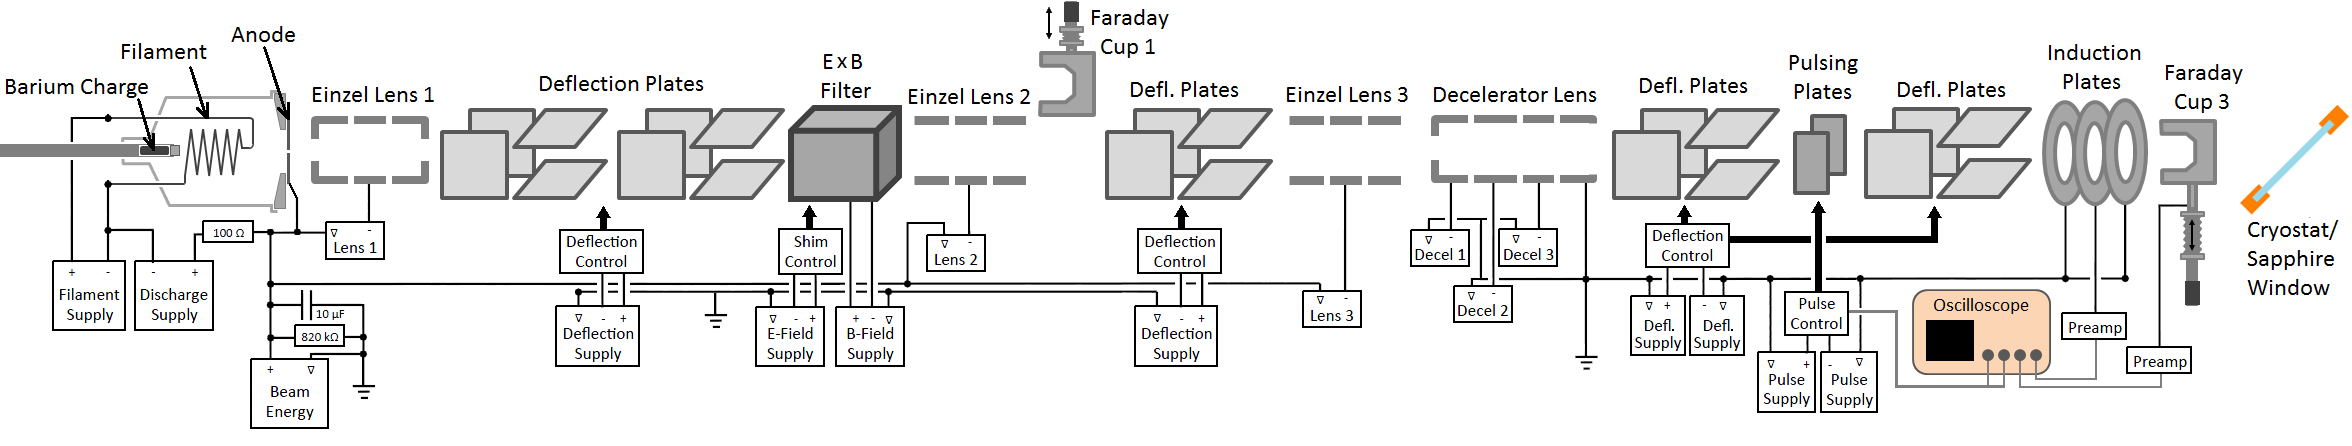
\includegraphics[angle=90,width=.25\textwidth]{figures/ionBeam.png}
                \caption{Ba\textsuperscript{+} ion beam.}
\label{fig:ionbeam}
\end{figure}

\subsection{Ion Source}

Ba\textsuperscript{+} ions are produced in a Model DCIS-101 Colutron ion gun system \cite{Colutron}.  The source is shown in Fig. \ref{fig:ionsource}.  A solid barium charge is placed into the hollowed end of a stainless steel rod, which is inserted into the discharge chamber, where it is heated by a filament.  The barium vaporizes, and escapes the hollowed rod around a loosely threaded set screw.  The source is designed to produce a discharge between the anode plate and the filament cathode, through an argon buffer gas leaked into the source chamber.  This controlled discharge would then also ionize atoms from the solid charge to produce the desired ion beam, and Ar ions would be filtered out.  However, to avoid contamination of the SXe matrix with residual Ar gas, the buffer gas was not used in this work.  Discharge can be maintained with Ba vapor alone.  The longevity of ion current from a single charge (at least several 10s of hours) suggests that Ba is coating the inner walls of the source chamber, and is heated enough to provide sufficient Ba pressure to support a discharge.  The discharge produces a plasma, containing barium ions, which escapes the chamber through a small hole in the anode, where it enters the acceleration region.  The acceleration potential applied is 2~kV, between the ion source anode and the first element of Einzel lens 1 (L1).  This lens approximately collimates the ion beam for passage through the E$\times$B velocity filter.

%This is supported by the observation of white oxidation of the inner source parts after a few minutes of exposure to air when opening the system.

\begin{figure} %[H]
        \centering
                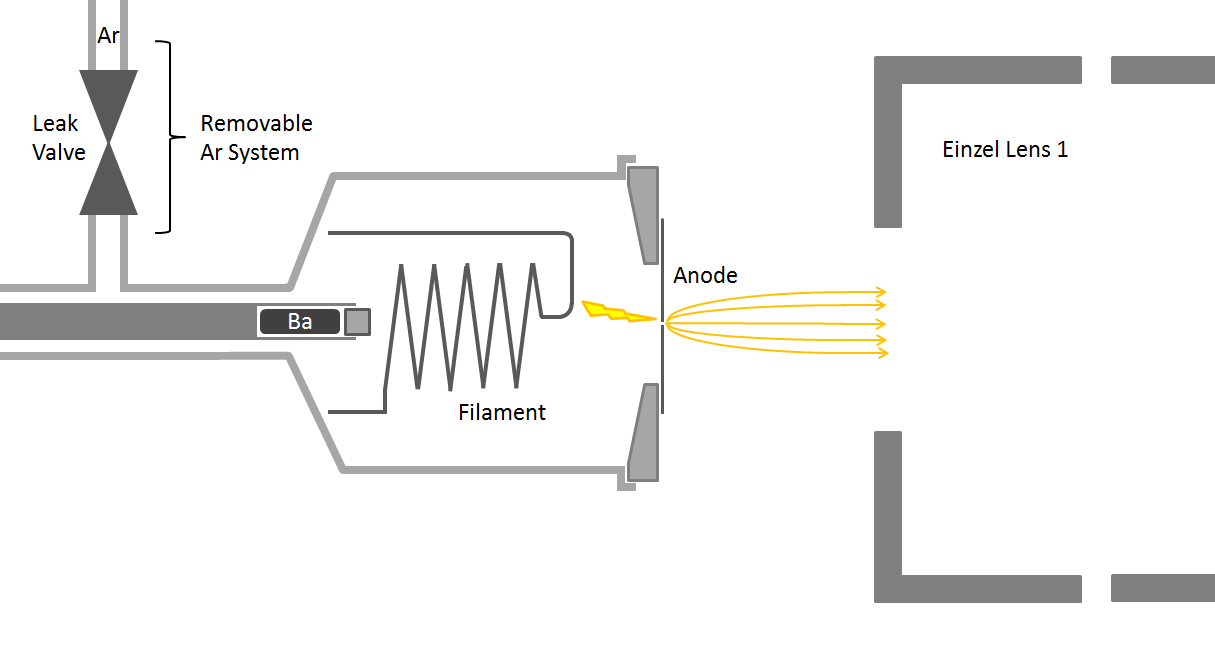
\includegraphics[width=.95\textwidth]{figures/ionSource.png}
                \caption{Ba\textsuperscript{+}/Ar\textsuperscript{+} ion source.}
\label{fig:ionsource}
\end{figure}

\subsection{E$\times$B Velocity Filter}

The E$\times$B velocity filter selects Ba\textsuperscript{+} by creating perpendicular electric and magnetic fields, which produce opposing forces on charged particles moving through the filter.  The opposing forces will be equal for ions with velocity $v = \frac{E}{B}$.  Since ion velocity is determined by mass ($m$), charge ($q$) and beam potential ($V$), the filter selects ions satisfying Eqn. \ref{eqn:massfilt}:

\begin{equation}
\frac{m}{q} = \frac{2 V B^{2}}{E^{2}}
\label{eqn:massfilt}
\end{equation}

\noindent
where $B$ and $E$ are the magnetic and electric fields, respectively.  Those fields are chosen such that Ba\textsuperscript{+} ions pass straight through.  Other ions will be deflected.  

The E$\times$B filter is shown in Fig. \ref{fig:exb}.  Electromagnets provide the vertical magnetic field.  Electrode plates and field-shaping guard rings provide the horizontal electric field.  The guard rings prevent a lensing and astigmatism effect from fringe fields of the plates \cite{Colutron}.

\begin{figure}[h]
        \centering
                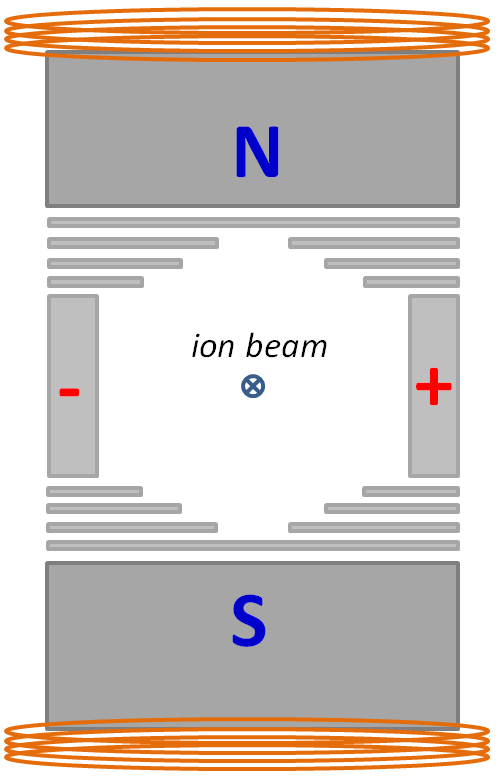
\includegraphics[width=.7\textwidth]{figures/ExB.png}
                \caption{Colutron E$\times$B ion velocity filter.}
\label{fig:exb}
\end{figure}

%\emph{\color{gray}If we need mass scans, we probably need to do new ones with a constant magnetic field, and Ar\textsuperscript{+} and Ba\textsuperscript{+} in same day.  Past scans were all over the place, partly because we were changing beam settings, but new peaks are not very consistent either.}
%To determine the mass components of the beam, the electric field can be scanned.  Mass scans of the Ba\textsuperscript{+} beam is shown in Fig. [ref mass scan fig], as well as of an Ar\textsuperscript{+} beam.  The known mass of Ar aids in calibrating the magnetic field, which differs from the calculation given by Colutron, likely due to hysteresis in the magnet.  \emph{\color{gray}The Ba\textsuperscript{+} peak agrees with the Ba mas s... }

\subsection{Other Beam Components}

The first three sets of deflection plates can be used for beam diagnostics, and are set to 0~V during normal operation.  The deflection plates just before the pulsing plates, H1 and V1, are set to constant values of +50~V and 0~V, respectively, which have been selected such that the beam, in both pulsing and continuous modes, can be deposited at the sapphire window for reasonable settings on the final deflection plates, H2 and V2.  As described in Section \ref{subsec:ionDepCal}, different settings in H2/V2 are required for peak ion current in Faraday cup 3 vs. peak deposit at the window.

Einzel lens 2 (L2) focuses the beam to pass through the aperture in the first element of the decelerator lens.  Einzel lens 3 (L3) is set to zero in this setup.  The decelerator lens can be used to vary Ba\textsuperscript{+} deposit energy, which was done in \cite{Shon}, but it in this work it acts as an Einzel lens with only the second element (D2) at voltage.  It focuses the beam near the sample and Faraday cup 3 (there is no Faraday cup 2 in this setup).  Faraday cup 3 measures the ion current during experiments, and is retracted when deposits are being made.  Calibration of deposits using Faraday cup 3 is described in Section \ref{subsec:ionDepCal}.  Faraday cup 1 can be used for beam diagnostics, and is usually retracted.  

To align the ion beam, L1 was first tuned to maximize ion current in Faraday cup 3, with L2, L3, and D2 set to zero.  Since cup 3 is about 2~m away from L1, this approximately collimates the beam for passage through the E$\times$B filter.  The optimal value for L1 was found to be around -400~V relative to the 2000~V beam energy \emph{\color{gray}consistent with Bill's SIMION -- show?}.  Next, L2 and D2 were fine-tuned together to achieve maximal current in cup 3.  Finally, the straightness of the beam was checked by peaking ion current with deflection plates H1 and V1 on cup 3, as well as on cup W, which is an additional Faraday cup attached to the coldfinger in place of the sapphire window.  Cup W is further described in Section \ref{subsec:ionDepCal}.

%L2 8.34 = 

\subsection{Ion Beam Pulsing}

When running in pulsing mode, the pulsing plates are normally set to 200~V and -200~V to deflect the beam, and are pulsed to 0~V for 1~$\mu$s to pass a short pulse of ions straight forward.  The pulsing circuit is shown in Fig. \ref{fig:pulse_circuit}.  Square waves, triggered by LabVIEW at 500~Hz, enter the circuit at (a). The transformed pulse triggers the MOSFET switch, which closes the circuit for the period of the pulse.

\begin{figure} %[h]
        \centering
                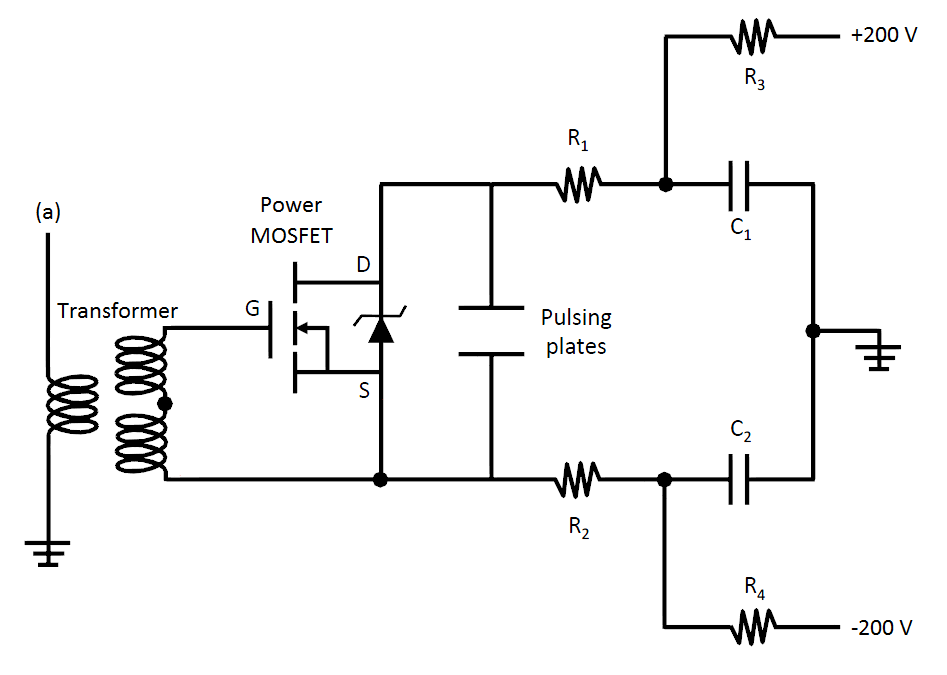
\includegraphics[width=.85\textwidth]{figures/pulsing_circuit.png}
                \caption{Pulsing circuit.  R$_{1}$ = R$_{2}$ = $470~\Omega$, R$_{3}$ = R$_{4}$ = 20~k$\Omega$, \newline C$_{1}$ = C$_{2}$ = 680~nF. \cite{Shon}}
\label{fig:pulse_circuit}
\end{figure}

The induction plates are used to observe pulses during a deposit.  Pulses just prior to a deposit can be observed by cup 3 (as well as the induction plates) for a measurement of ion current in the pulses.  eV Products pre-amplifiers convert the ion current to voltage signals, which are recorded on a digital oscilloscope.  An example of raw oscilloscope traces of Faraday cup 3 and induction plate signals are shown in Fig. \ref{fig:pulse_raw_shaped}(a).  The pre-amp output voltage is related to the input current according to Eqn. \ref{eqn:preamp}:

\begin{equation}
I = \frac{-(V_{out} + R_{1} C \frac{dV_{out}}{dt})}{R_{1} M}
\label{eqn:preamp}
\end{equation}

\noindent
$R_{1} C$ and $R_{1} M$ are determined by putting a known square pulse into the pre-amp.  First, the time constant of an exponential fit to the signal decay determines $R_{1} C$, and then $R_{1} M$ is determined by matching this shaped signal to the original square pulse.  Actual currents in the induction plates and cup 3 are shown in Fig. \ref{fig:pulse_raw_shaped}(b).  The induction signal is positive as ions are approaching the sensitive plate, and an equal but negative signal is seen after the ions pass through.  The Faraday cup stops the ions, so it produces only a positive induction signal as ions approach it.

\begin{figure} %[H]
        %\centering
        %\begin{subfigure}
                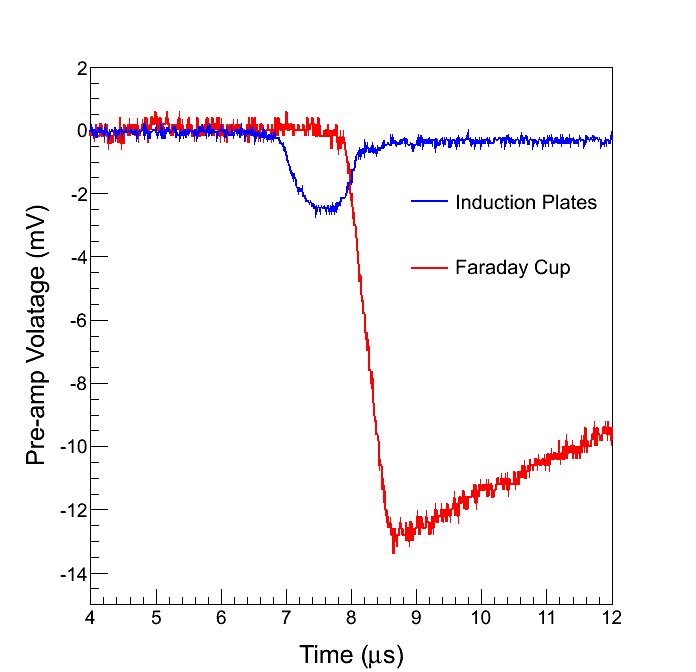
\includegraphics[width=.49\textwidth]{figures/pulse_ind_cup3_raw.png}
                %\caption{barf}
%        %\end{subfigure}
        %\begin{subfigure}
                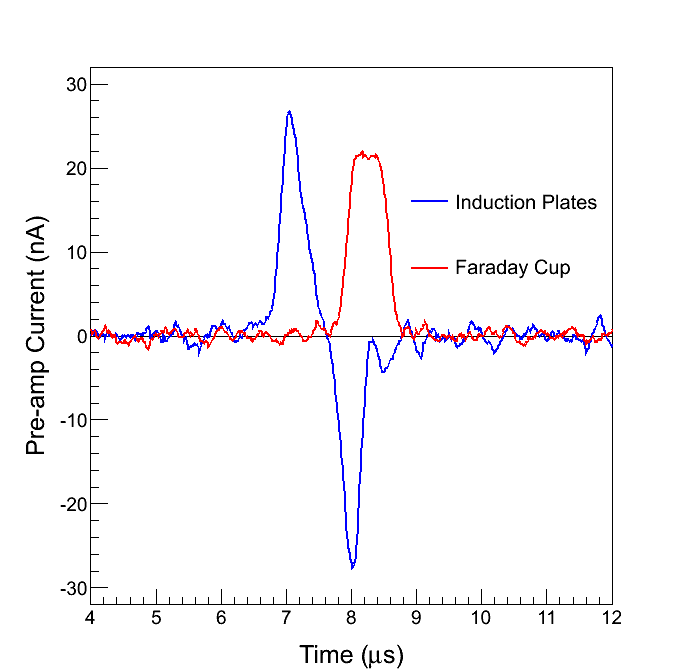
\includegraphics[width=.49\textwidth]{figures/pulse_ind_cup3_shaped.png}
                \caption{Raw (a) and shaped (b) pulse signals from induction plates and cup 3.  The raw induction signal appears small because it is a less sensitive pre-amp (accounted for in shaping).}
        %\end{subfigure}
        \label{fig:pulse_raw_shaped}
\end{figure}

Pulsing data also provides confirmation that the beam is composed of Ba\textsuperscript{+}.  The time between the center of the pulsing plate voltage overlap and the center of the pulse measured by the Faraday cup, along with a measurement of the distance traveled, provides a velocity measurement of the ions.  This distance was measured to be 31.5 $\pm$ 0.5~cm from the center of the pulsing plates to the Faraday cup, and time-of-flight data, e.g. Fig. \ref{fig:pulses_ArBa}, give 39.8 $\pm$ 3.4~amu for Ar\textsuperscript{+} and 136.8 $\pm$ 6.3~amu for Ba\textsuperscript{+}, including an uncertainty on the time of flight of $\pm$ 0.1~$\mu s$.

\begin{figure}[h]
        \centering
                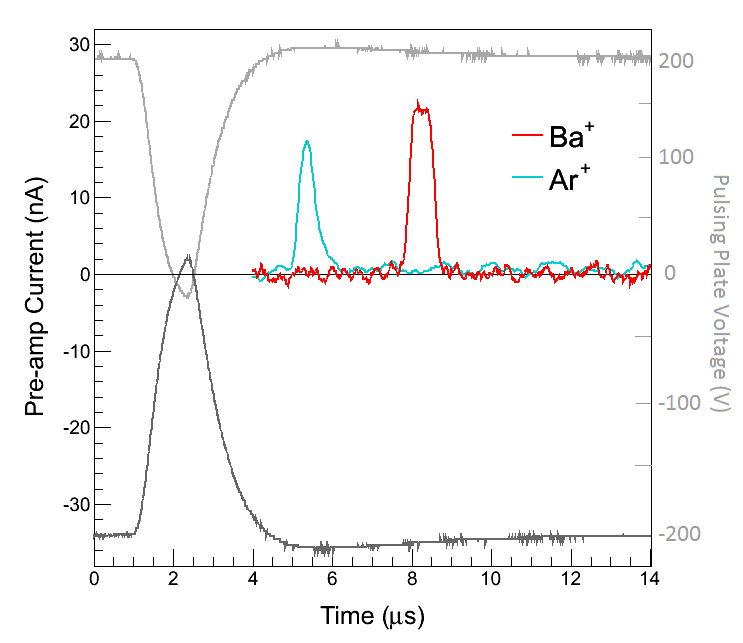
\includegraphics[width=.7\textwidth]{figures/pulses_BaAr.png}
                \caption{Arrival time of pulses at cup 3 vs. time of pulsing plate signal (black (+) and gray (-)) for Ar\textsuperscript{+} and Ba\textsuperscript{+}.}
\label{fig:pulses_ArBa}
\end{figure}

\subsection{Calibration of Ion Deposit}
\label{subsec:ionDepCal}

To calibrate the signal at cup 3 to an ion density at the sapphire window, another Faraday cup (cup W) is attached to the cold finger in place of the sapphire window.  The ratio of between ion current in cup 3 and cup W is measured ($\equiv f$).  Then, knowing the radius of the entrance aperture in cup W lets one determine the ion density per pulse at the sapphire window:

\begin{equation}
\frac{ions}{pulse \times m^{2}} = \frac{Q f}{e A}
\label{eqn:ion_density}
\end{equation}

\noindent
where $Q$ is the charge/pulse at cup 3, $A$ is the area of cup W, and $e$ is the elementary charge.  The voltages on the final deflection plates H2 and V2 are also determined to optimize the signal in cup W.  In later experiments, these differed from the values for maximum cup 3 signal by about 70~V in H2 and 60~V in V2, corresponding to about 4~mm in x and y position at cup W, indicating that some drift in optimal ion beam component settings occurred over time.

\section{Ba Getter Source}

A BaAl$_{4}$ getter, manufactured by SAES, can be inserted on a bellows to emit toward the sapphire window, shown in Fig. \ref{fig:endOfBeamBa}.  When heated, the getter emits neutral Ba with minimal Ba\textsuperscript{+}.  Getters were used extensively in previous work \cite{Brian} for measuring the absorption of Ba in SXe with large Ba deposits, and in identifying emission peaks.  A getter was used briefly in this work in identifying the 619-nm fluorescence peak, as described in Section \ref{sec:619identification}.  The barium getters used in \cite{Brian} were exothermic BaAl$_{4}$-Ni flash getters.  The getter used here is an endothermic BaAl$_{4}$ type, designed for more controlled Ba emission.  

%no evidence is provided in Brian's thesis, nor Shon's, and I don't see anything on the SAES website

\begin{figure} %[h]
        \centering
                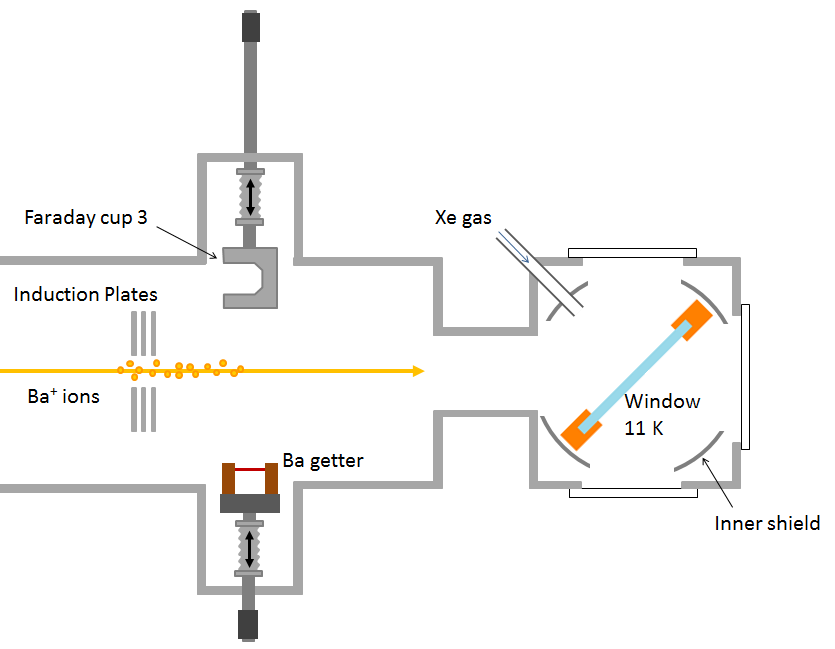
\includegraphics[width=.75\textwidth]{figures/window_etc_justBa.png}
                \caption{Apparatus near sapphire window, including Ba getter, Faraday cup 3, induction plates, and Xe gas inlet.}
\label{fig:endOfBeamBa}
\end{figure}

%\begin{figure} %[h]
%        \centering
%                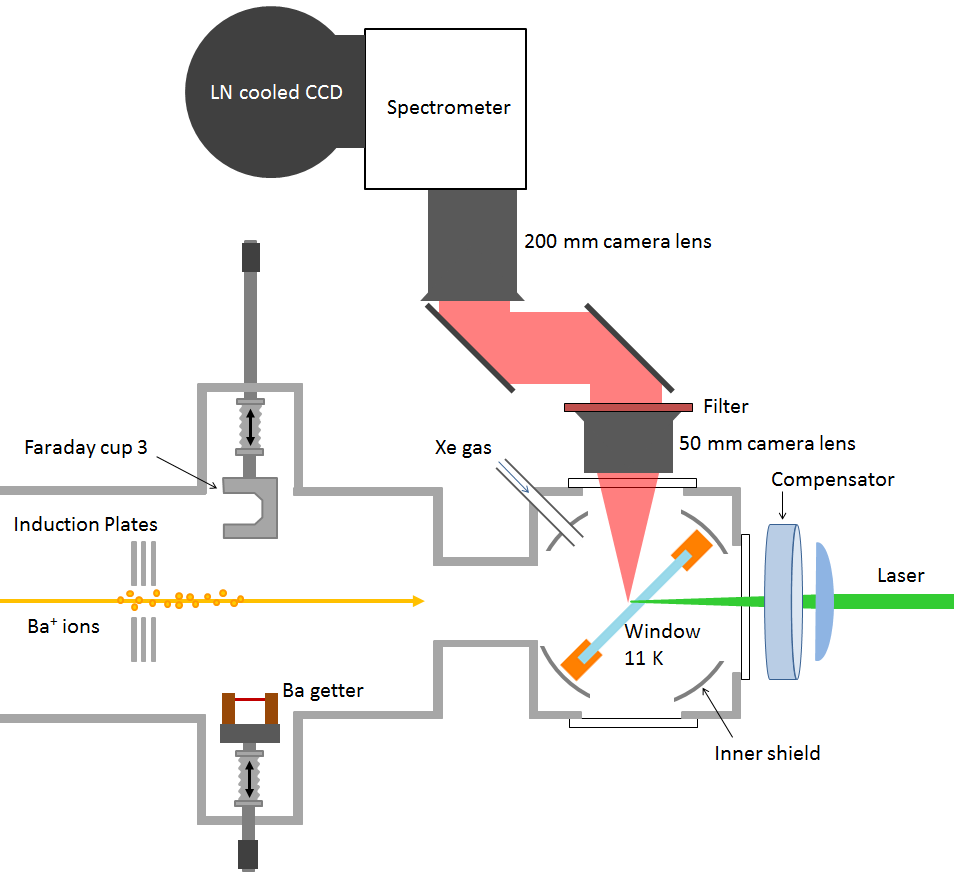
\includegraphics[width=.9\textwidth]{figures/window_etc.png}
%                \caption{Apparatus in spectroscopy region, including Ba getter, Faraday cup 3, induction plates, and optics for excitation, fluorescence collection, spectroscopy and detection.}
%\label{fig:endOfBeam}
%\end{figure}

\section{Sample Deposition}
\label{sec:deposition}

The Ba\textsuperscript{+}/Ba is co-deposited with ultra-pure Xe gas onto a cold sapphire window.  Sapphire has good thermal conductivity at low temperature and good optical transparency in the visible.  The window is held in a copper mount attached to a coldfinger and is tilted at 45$^{\circ}$ to allow access of the ion beam and Xe gas, as well as the excitation laser and collection optics.  To begin a deposit, Xe gas is flowed toward the window via a leak valve.  Cup 3 is then retracted and the ion beam is pulsed, depositing Ba\textsuperscript{+} ions into the SXe matrix as it grows.  Cup 3 is then replaced, and the Xe leak stopped.

\begin{figure} %[h]
        \centering
                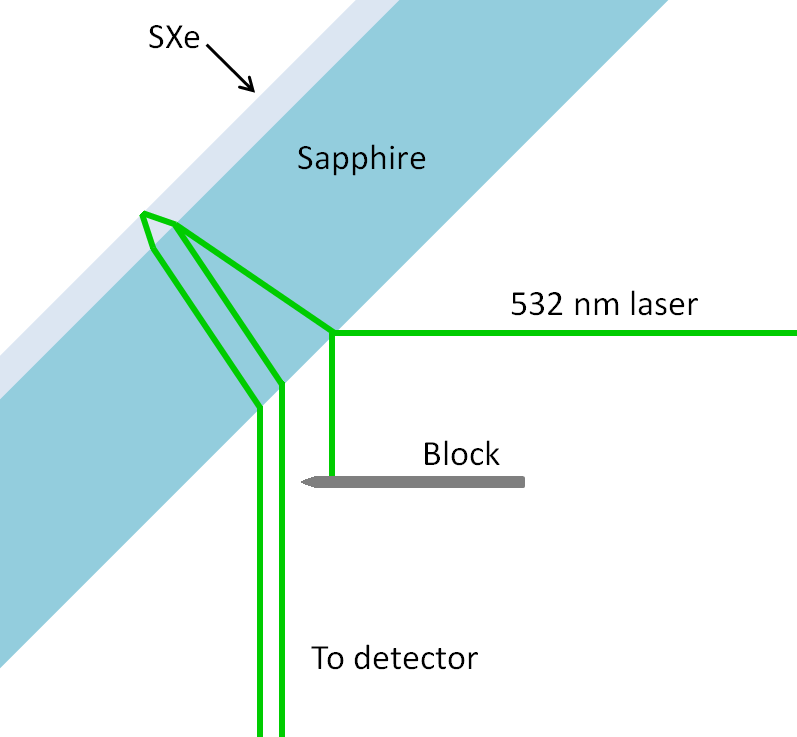
\includegraphics[width=.4\textwidth]{figures/fringe_setup.png}
                \caption{Setup for measuring SXe deposition rate by interference fringes.}
\label{fig:fringe_setup}
\end{figure}

\begin{figure} %[h]
        \centering
                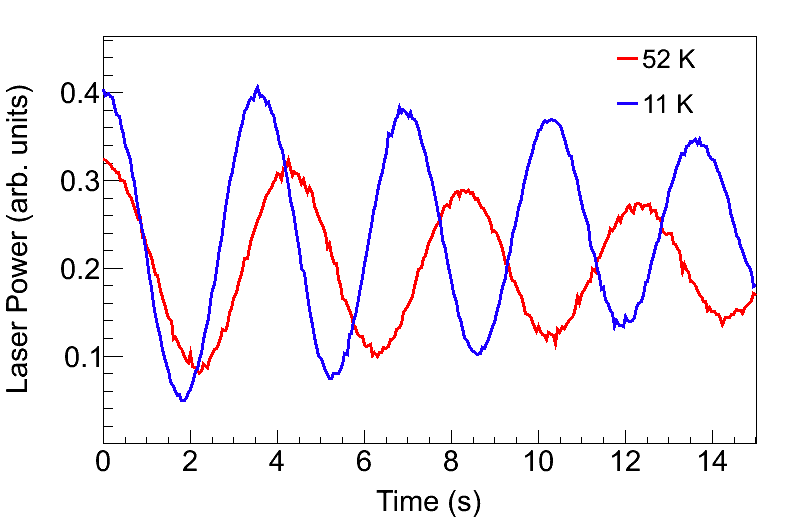
\includegraphics[width=.5\textwidth]{figures/fringes_52K_vs_11K.png}
                ~
                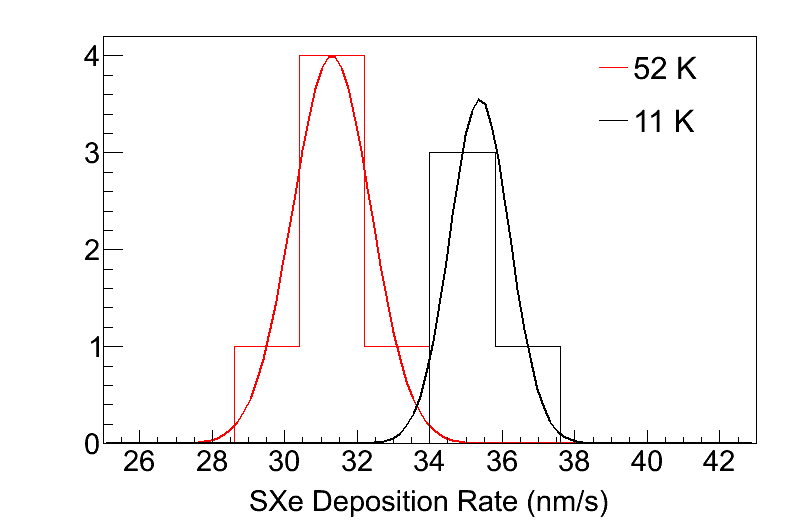
\includegraphics[width=.5\textwidth]{figures/fringes_52K_vs_11K_statistics.png}
                \caption{Interference fringes for the same Xe gas leak rate deposited on the sapphire window at 11~K and at 52~K.}
\label{fig:fringes_52K_vs_11K}
\end{figure}

SXe matrix deposition rate can be measured by interference fringes in a laser reflected against the front surface of the sapphire window, as shown in Fig. \ref{fig:fringe_setup}.  Fringes for SXe deposition at 52~K and 11~K are shown in Fig. \ref{fig:fringes_52K_vs_11K}(a) for the leak rate used in this work.  The refractive index of SXe has a negligible dependence on temperature between 50~ and 30~K \cite{SXeIndex}, so these can be compared directly.  A distribution of SXe deposition rate measurements from several deposits is shown in Fig. \ref{fig:fringes_52K_vs_11K}(b).  A somewhat lower rate is observed at 52~K, $31.3 \pm 0.44(\text{stat}) \pm 0.31(\text{sys})$~nm/s, vs. $35.4 \pm 0.41(\text{stat}) \pm 0.35(\text{sys})$~nm/s at 11~K.  Statistical errors are $\sigma / \sqrt{N}$ where $\sigma$ is the standard deviation of the Gaussian fits to the distributions in Fig. \ref{fig:fringes_52K_vs_11K}(b), and $N$ is the number of entries.  Systematic errors come from propagating an uncertainty on the angle between the laser and sapphire window of $\pm 2^{\circ}$.

\begin{figure} %[h]
        \centering
                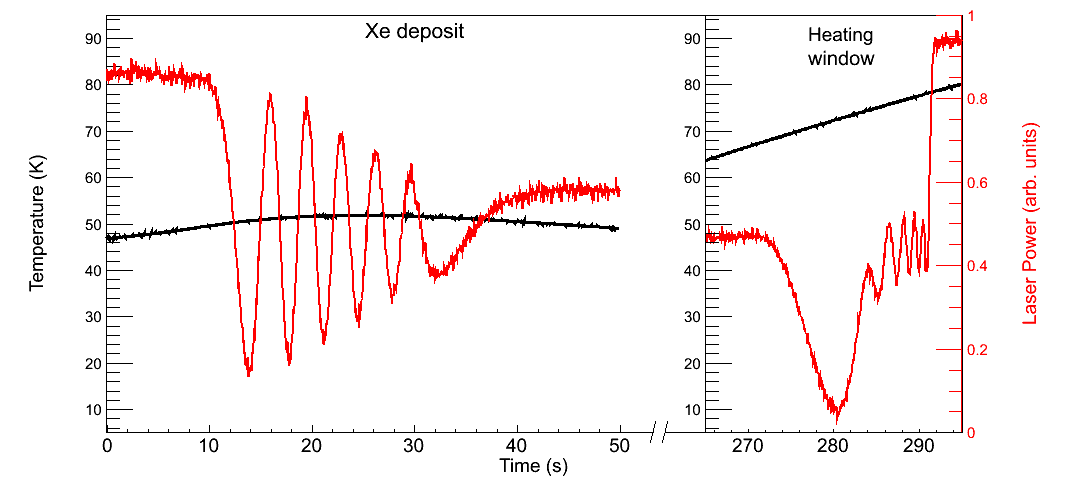
\includegraphics[width=.9\textwidth]{figures/fringes_dep_and_melt.png}
                \caption{(a) Interference fringes of a deposit at 52~K and of its subsequent evaporation when heating the sapphire window, and (b) distribution of SXe deposition rates calculated from fringe period of several measurements.}
\label{fig:fringes_melt_withDep}
\end{figure}

To evaporate a sample, the window is heated to 100~K.  Fringes appear during this process as well.  The full set of fringes for a deposit at 52~K and its evaporation when heated is shown in Fig. \ref{fig:fringes_melt_withDep}, along with the window temperature.  This shows that the SXe evaporates between 73~K and 78~K.  The same number of fringes appear in the deposit and the evaporation, indicating that the lower deposition rate at around 50~K is not due to simultaneous evaporation.  The variance in temperature during the deposit is due to the heater cycle.  Note that these Xe deposits were longer than for a typical deposit during a fluorescence experiment, in order to observe several fringes.

%quadrature errors: 0.54 for 52 K and 

\section{Laser Excitation}

\begin{figure} %[h]
        \centering
                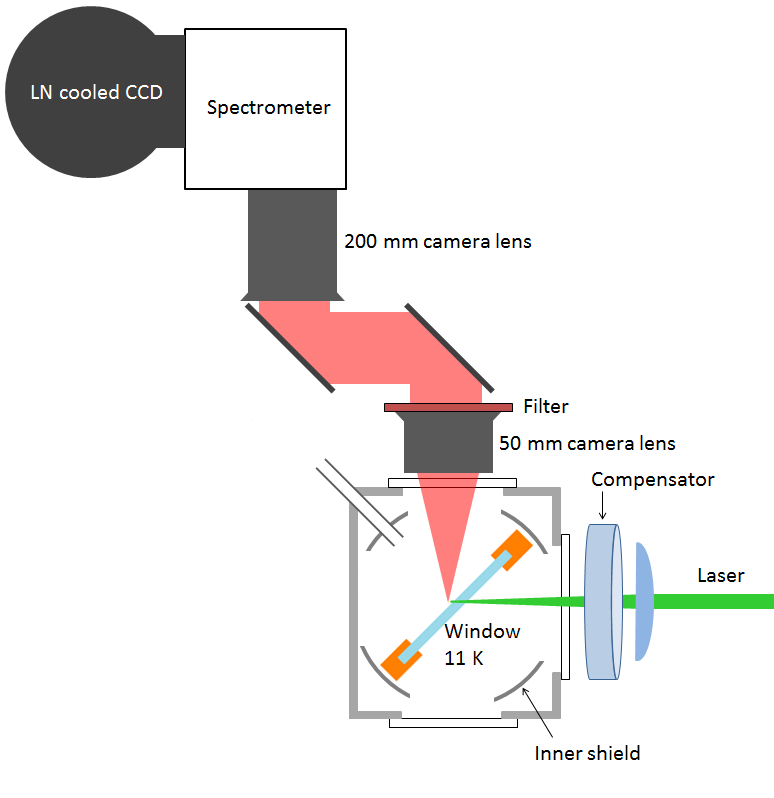
\includegraphics[width=.7\textwidth]{figures/window_etc_justOptics.png}
                \caption{Apparatus in spectroscopy region, including optics for excitation, fluorescence collection, spectroscopy and detection.}
\label{fig:endOfBeamOptics}
\end{figure}

Green to yellow laser excitation is done with a Coherent 599 dye laser, pumped by the 514-nm line of a Lexel 3500 Ar ion laser.  Rhodamine 110 (R110) dye is used for the 542 - 566~nm wavelength range, and Rhodamine 6G (R6G) for the 567 - 590~nm range.  Another Coherent 599 dye laser with Coumarin 480 (C480) dye is used for blue excitation, which is pumped by a Kr ion laser.  The Coherent 599 dye lasers are used with birefringent filters for wavelength tuning, but without etalons, since the broad absorption of Ba in SXe does not require single-mode laser excitation.

\begin{figure} %[h]
        \centering
                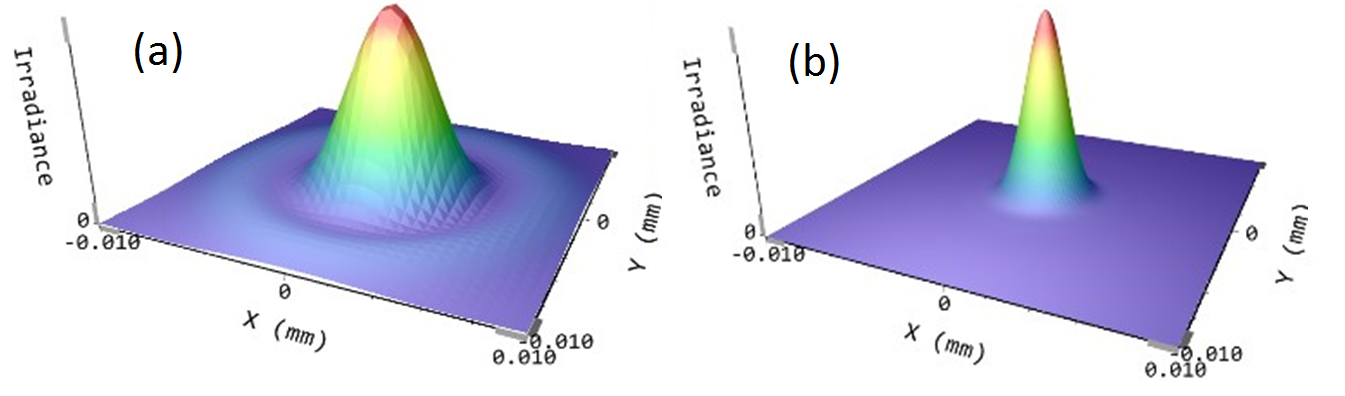
\includegraphics[width=.7\textwidth]{figures/DFairbank_aber.png}
                \caption{Calculated minimum laser spot size distributions, with wavelength 570~nm and unfocused waist w = 7~mm, for (a) bi-convex f = 7~cm lens, and (b) aspherical f = 7.9~cm lens.}
\label{fig:DFairbank}
\end{figure}

A lens focuses the laser into the cryostat from the side, shown in Fig. \ref{fig:endOfBeamOptics}.  Initial work, spectroscopy (Chapter 4) and some imaging, was done using a bi-convex, which produced spherical aberration near the laser focus.  This effect does not affect the results in Chapter 4, where semi-focused beam waists of 100-1000~$\mu$m were used.  However, spherical aberrations caused the minimum beam waist to be about twice that of the diffraction limit.  To approach the diffraction limit in imaging small numbers (Chapter 5), a 7.9-cm focal length aspherical lens was used.  A comparison of the minimum spot sizes for these two lenses, calculated by David Fairbank at Thorlabs, is shown in Fig. \ref{fig:DFairbank}.

To correct for astigmatism introduced by the tilted sapphire window, compensating astigmatism is introduced by a fused silica optical flat of 1~cm thickness, placed after the lens, tilted on the y-axis (the laser is along the z-axis, and the sapphire window is tilted on the x-axis).  The proper angle for the compensator was determined to be about 10$^{\circ}$ from normal by a ray matrix calculation \cite{raymatrix}.  The effect of the SXe layer is negligible since its thickness is only about half a micron in a typical fluorescence experiment.  With the compensator, overlapping minimum spot sizes of 2.06~$\mu$m and 2.66~$\mu$m are calculated for x and y, respectively.  To observe the astigmatism and the effect of the compensator, the relative position of the x- and y-focus was observed by imaging 619-nm Ba fluorescence from a large deposit of Ba\textsuperscript{+} in SXe, with a varying laser focus.  For each z-position of the laser focusing lens, an image was taken, and a 2D Gaussian fit determined the x and y beam waists, w$_{\text{x}}$ and w$_{\text{y}}$.  Example fits to the 619-nm fluorescence for three laser focus positions, using the astigmatism compensator at 10$\pm 1^{\circ}$, are shown in Fig. \ref{fig:astig}(a,b,c).  Gaussian fit values for w$_{\text{x}}$ and w$_{\text{y}}$ are plotted vs. laser focus position with (d) no compensator, and with the compensator at (e) 10$\pm 1^{\circ}$, (f) 13$\pm 1^{\circ}$, and (g) 11$\pm 1^{\circ}$.  With no compensator (d), the focal positions for x and y are measured to be 127.6$ \pm 2.5$~$\mu$m apart.  10$\pm 1^{\circ}$ (e) and 13$\pm 1^{\circ}$ (f) can be seen to under- and over-shoot the optimal angle, respectively.  11$\pm 1^{\circ}$ (g), which was used in imaging experiments, is near optimal, i.e. the x and y foci are consistent to within 45~$\mu$m.  \emph{\color{gray}A systematic uncertainty... on the beam size is then obtained ... leading to a focused laser spot of ?? $\pm$ ?? $\mu$m\textsuperscript{2} [get this uncertainty from error propagation of angle(s) through gaussian beam ray matrix}

%\emph{\color{gray}which is consistent with the calculated value of {\color{red}??}~$\mu$m from...}

\begin{figure} %[H]
        \centering
                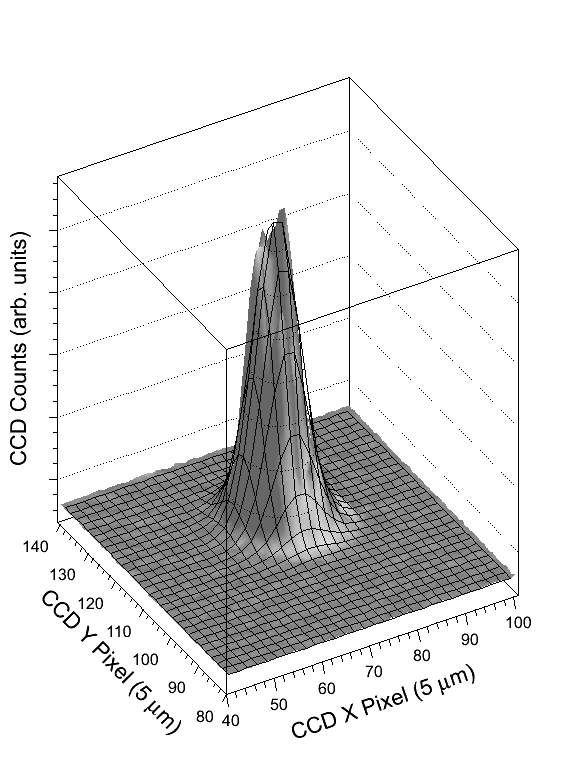
\includegraphics[width=.33\textwidth]{figures/astig_thesis_2Dgaus_run35.png}
                ~
                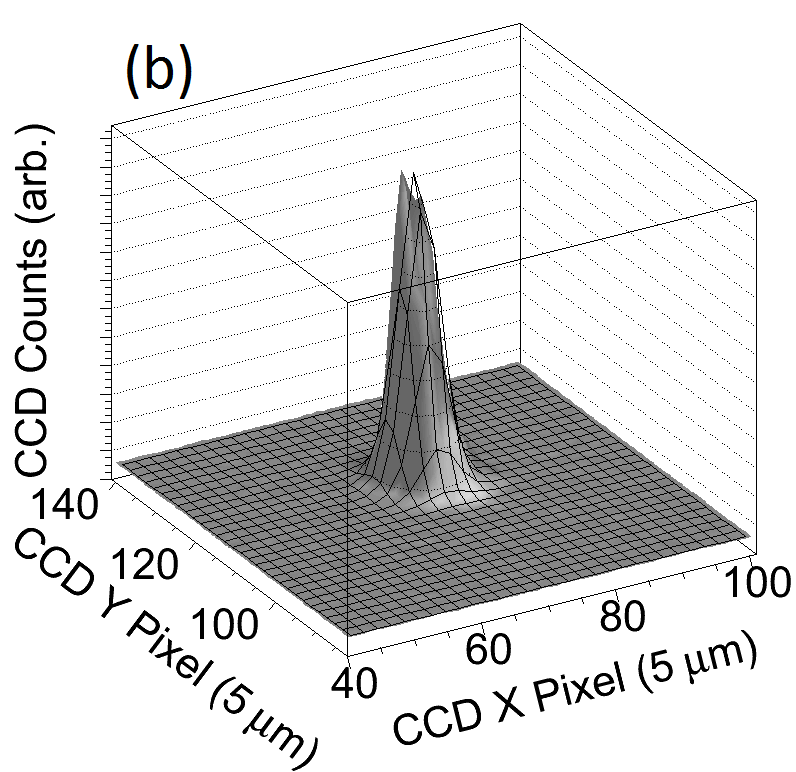
\includegraphics[width=.33\textwidth]{figures/astig_thesis_2Dgaus_run39.png}
                ~
                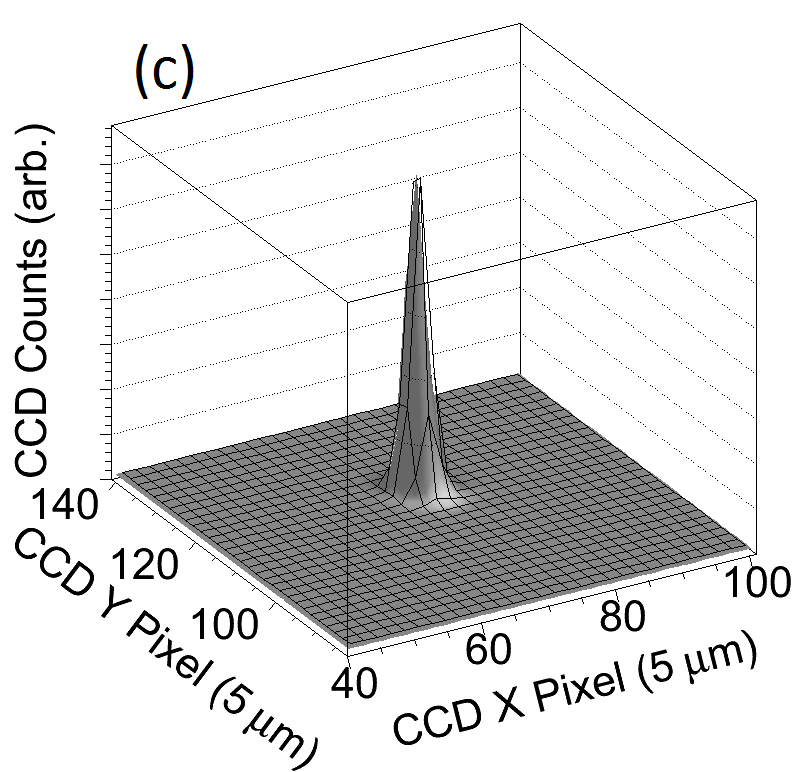
\includegraphics[width=.33\textwidth]{figures/astig_thesis_2Dgaus_run43.png}
                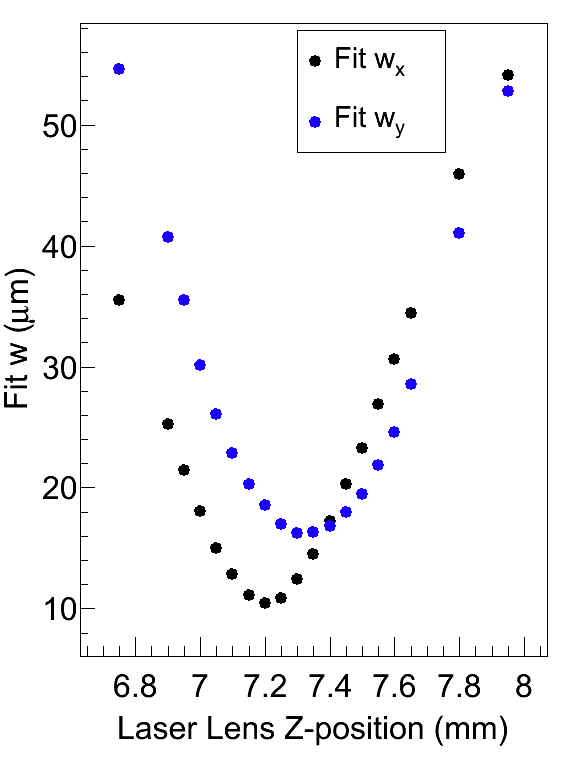
\includegraphics[width=.45\textwidth]{figures/astigcorr_curve_no-corr_806.png}
                ~
                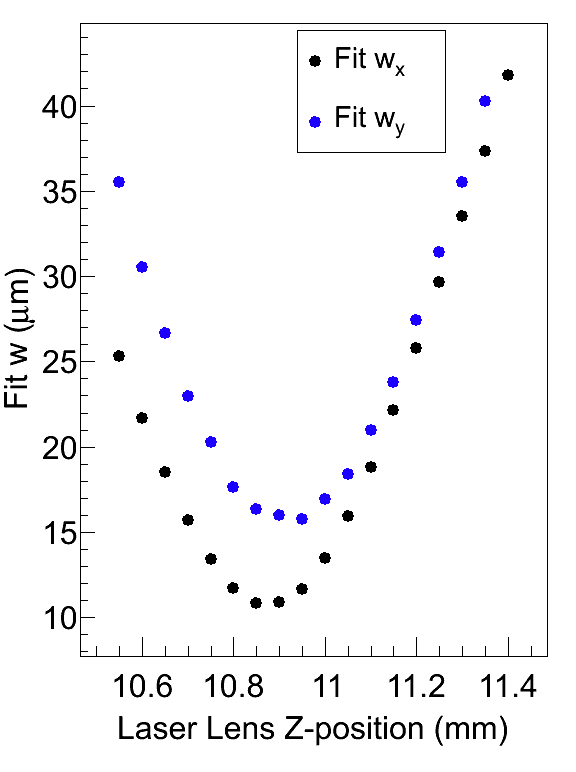
\includegraphics[width=.45\textwidth]{figures/astigcorr_curve_corr_10deg.png}
                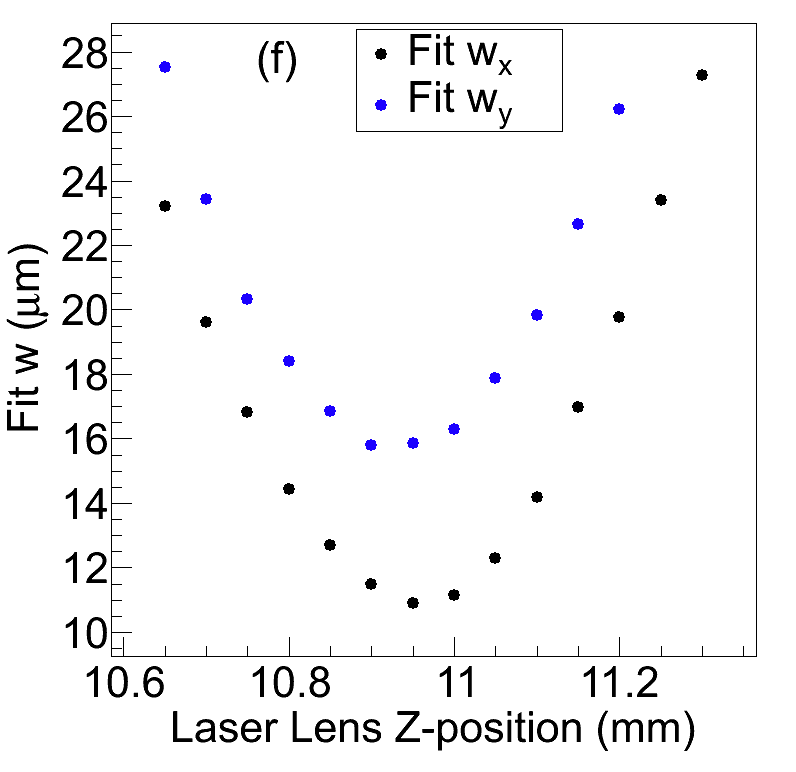
\includegraphics[width=.45\textwidth]{figures/astigcorr_curve_corr_13deg.png}
                ~
                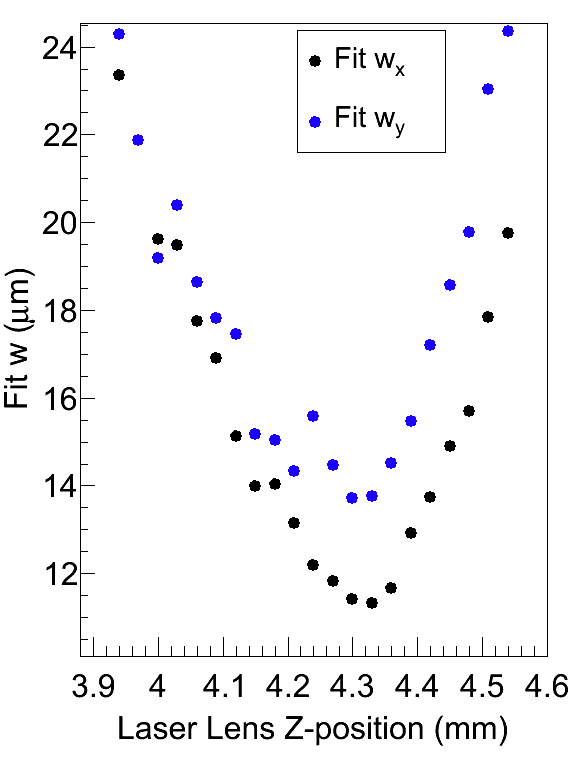
\includegraphics[width=.45\textwidth]{figures/astigcorr_curve_corr_9-16.png}
                \caption{Example 2D Gaussian fits (black grid lines) with varying laser focus (a,b,c), and fit waists  w$_{\text{x}}$ (black) and  w$_{\text{y}}$ (blue) vs. laser focus lens position with (d) no compensator, and with compensator at about (e) 10$^{\circ}$, (f) 13$^{\circ}$, and (g) 11$^{\circ}$.}
\label{fig:astig}
\end{figure}

%[waist measurements? -- apply calibration uncertainty to the good motor-stage ones]

%show measurements of astig. w/ and w/o compensator.?  8-7 prolly best so far

%Astigmatism in the laser itself was measured to be consistent with zero. (pg. 24 of Chris's book)
\section{Collection Optics}
\label{sec:collection}

Fluorescence is collected above the cryostat (Fig. \ref{fig:endOfBeamOptics}).  A 50~mm Nikon camera lens collimates the light, and a fluorescence filter sits on top of it.  A band-pass filter is used for imaging, and a Raman filter was used for spectroscopy.  The fluorescence then reflects off two steering mirrors, and is imaged by a 200~mm Nikon camera lens onto a Roper Scientific liquid-nitrogen-cooled CCD, with a magnification of 4.  The CCD has a quantum efficiency of 90\% in the visible, and in slow ADC mode, records one count per two photons collected.  At the set point of -100~$^{\circ}$C, dark counts are negligible.

The CCD has a removable Princeton Instruments imaging spectrometer.  With this attached, the 200~mm camera lens focuses the light onto an inlet slit, which is then imaged by the spectrometer onto the CCD after reflecting off a diffraction grating.  The 0-order reflection of the grating provides an image for alignment, and the grating can be tilted to distribute the 1\textsuperscript{st}-order reflection across the horizontal CCD pixels for doing spectroscopy.

When a 1" diameter filter is used, the imaging system has a solid angle collection of about 1.5\%.  Each additional component in the collection optics, listed in Table \ref{table:colleff}, contributes some loss, resulting in a total collection efficiency ($\epsilon_{c}$) of $2.4 \times 10^{-3}$ with the spectrometer, and $4.8 \times 10^{-3}$ without.  The spectrometer also limits the system to an f-number of 4, though this is not limiting in this setup.

\begin{table} [!htbp]
\caption{Factors contributing to optical collection efficiency.  Total $\epsilon_{c}$ includes 1.5\% solid angle collection.}
\label{table:colleff}
\begin{tabular}{l l l}
Component & Efficiency & \\
\hline
Cryostat Window & 0.99 & \\
Camera Lens 50~mm & 0.89 & \\
Camera Lens 200~mm & 0.91 & \\
Steering Mirrors ($\times 2$) & 0.95 & \\
CCD Quantum Efficiency & 0.90 & \\
Filter & 0.98 & \\
Counts per Photon (CCD) & 0.5 & $\epsilon_{c}\text{(w/o spectrom.)} = 4.8 \times 10^{-3}$\\
\hline
Spectrometer & 0.5 & $\epsilon_{c}\text{(w/ spectrom.)} = 2.4 \times 10^{-3}$\\
\end{tabular}
\end{table}

%Spectrom. Mirrors ($\times 2$) & {\color{red}??} & \\
%Diffraction Grating & 0.5 & $\epsilon_{c}\text{(w/ spectrom.)} = ${\color{red}??}\\

To limit laser exposure to only the time of CCD exposure, a laser shutter was linked to the camera exposure with a LabVIEW program.  This program also recorded laser power via a calibrated pickoff, as well as the temperature of the coldfinger near the sapphire window during observation.

\section{Vibrations and Effective Laser Region}

\begin{figure} %[H]
        \centering
                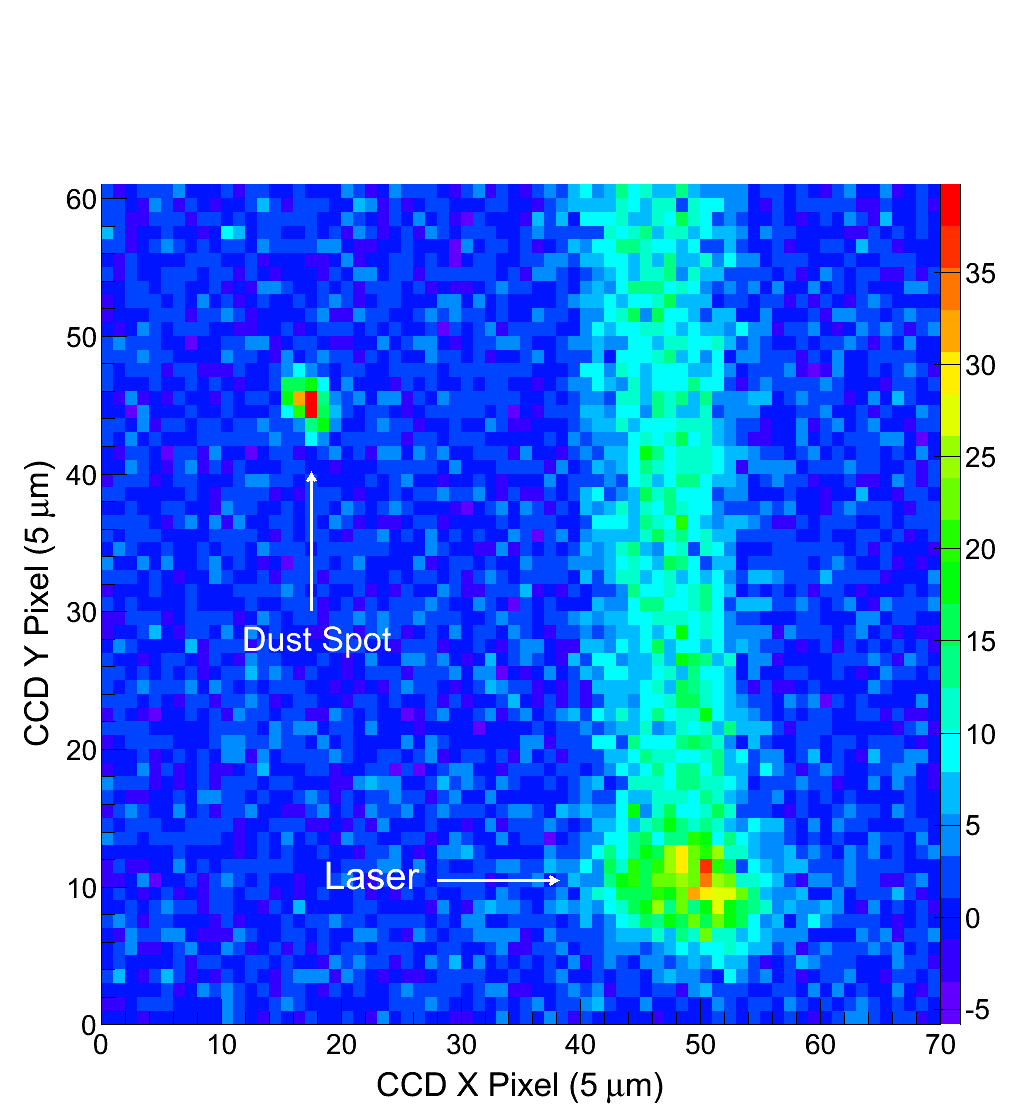
\includegraphics[width=.6\textwidth]{figures/image_dustspot.png}
                \caption{Example image of dust spot and laser during observation of cryostat vibrations.}
\label{fig:dustspot}
\end{figure}

Relative vibrations between the laser and sapphire window affect the number of Ba atoms exposed, increasing the effective laser spot size.  This was studied by observing the position of a ``dust spot" (a highly scattering feature on the sapphire window) relative to the position of the laser in an image on time scales down to 50~ms.  An example of an image from this experiment is shown in Fig. \ref{fig:dustspot}.  The 570-nm dye laser was somewhat de-focused, and the dust spot was illuminated by a de-focused 657~nm diode laser. For each frame, 2D Gaussian functions were fit to locate the center of the laser spot and the dust spot in order to measure their relative position.  The fit for the laser spot was restricted in y so that it was not affected by the bulk sapphire fluorescence path.  The distances in x and y between the dust spot and laser are plotted for each 50-ms snapshot in Fig. \ref{fig:cryovibe2D}(a).  The distribution shows a correlation between x and y.  To calculate an effective laser spot size due to this vibration, each difference (x,y) between laser and dust spot was used as the center of a 2D Gaussian, each with w$_{x} = 2.06~\mu$m and w$_{y} = 2.66~\mu$m to represent the laser spot.  Such Gaussian functions were summed for all points to produce a distribution of summed laser exposure, shown in Fig. \ref{fig:cryovibe2D}(b).  The total area enclosed by a 1/e contour then represents the effective area.  Since x and y movement are correlated, and since the movement is sinusoidal, the effective area is only about 5$\times$ the real laser spot size, and the effective laser region is about 40~$\mu$m$^{2}$.

%The difference between dust spot and laser positions is plotted in {\color{red}Fig. [fig vibe vs. time with sine fit]} for both x and y.  Each exposure in this plot is 50~ms, though readout time and camera shutter compensation time result in x~s between frames.  The best fit of a sine function results in a vibration frequency of x~Hz.  This is consistent with the audible frequency of the cryostat He pump.
%...could do this for rotated

\begin{figure} %[H]
        \centering
                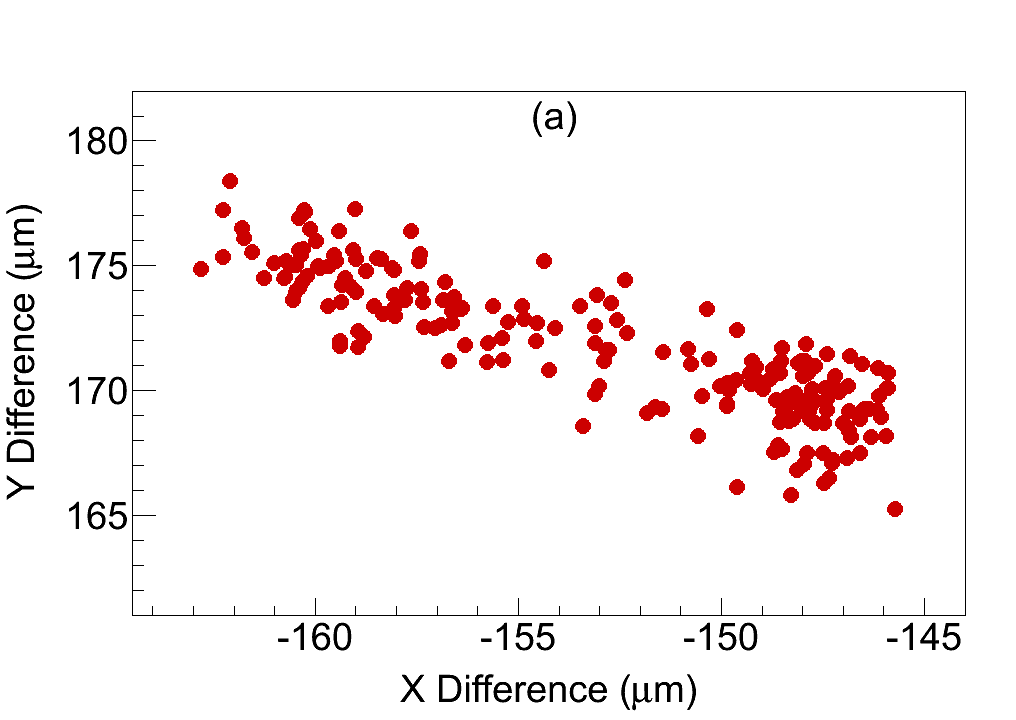
\includegraphics[width=.5\textwidth]{figures/cryovibes_a.png}
                ~
                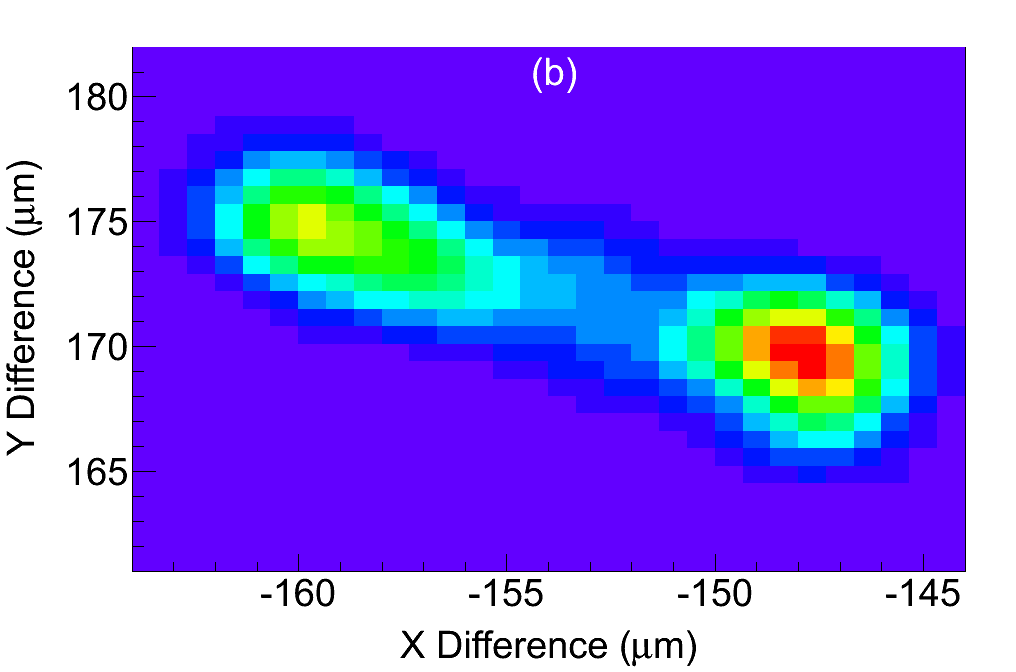
\includegraphics[width=.5\textwidth]{figures/cryovibes_b.png}
                \caption{Cryostat vibration measurements based on relative position of dust spot vs. laser on sapphire window in 50-ms snapshots (a), with 2D Gaussians overlain on each point to represent total laser exposure vs. position (b).}
\label{fig:cryovibe2D}
\end{figure}

The aforementioned is the most concerning vibration to understand.  Vibration of the laser itself is included in that study.  Vibration of the collection optics will affect the imaging resolution, but not the number of atoms being observed.  These vibrations were minimized by stable mounts.

\section{Laser Scanning}
\label{sec:laserscanning}

In order to obtain images of separated single atoms, the laser focusing lens is attached to motorized translation stages which scan the laser position by scanning the lens in x and y, shown in Fig. \ref{fig:laserStages}.  These stages sit atop a manual z-translation stage for laser focusing.  An extension of the aforementioned LabVIEW program coordinates movement of these stages such that x or y position is stepped in between CCD frames, and each frame then corresponds to a position in a laser scan grid.

The stages used in this work were Newport AG-LS25, which are driven by piezoelectric motors, but without accurate position feedback.  As a result, some inconsistency in position reproducibility was observed.  The position of the focused laser, measured by the center of a 2D Gaussian fit to the image of the laser spot, is shown in Fig. [fig laser grid] for ...

%\emph{\color{gray}Show data on steps and reproducibility -- say this isn;t good and new stages will be used later.}

\begin{figure} %[h]
        \centering
                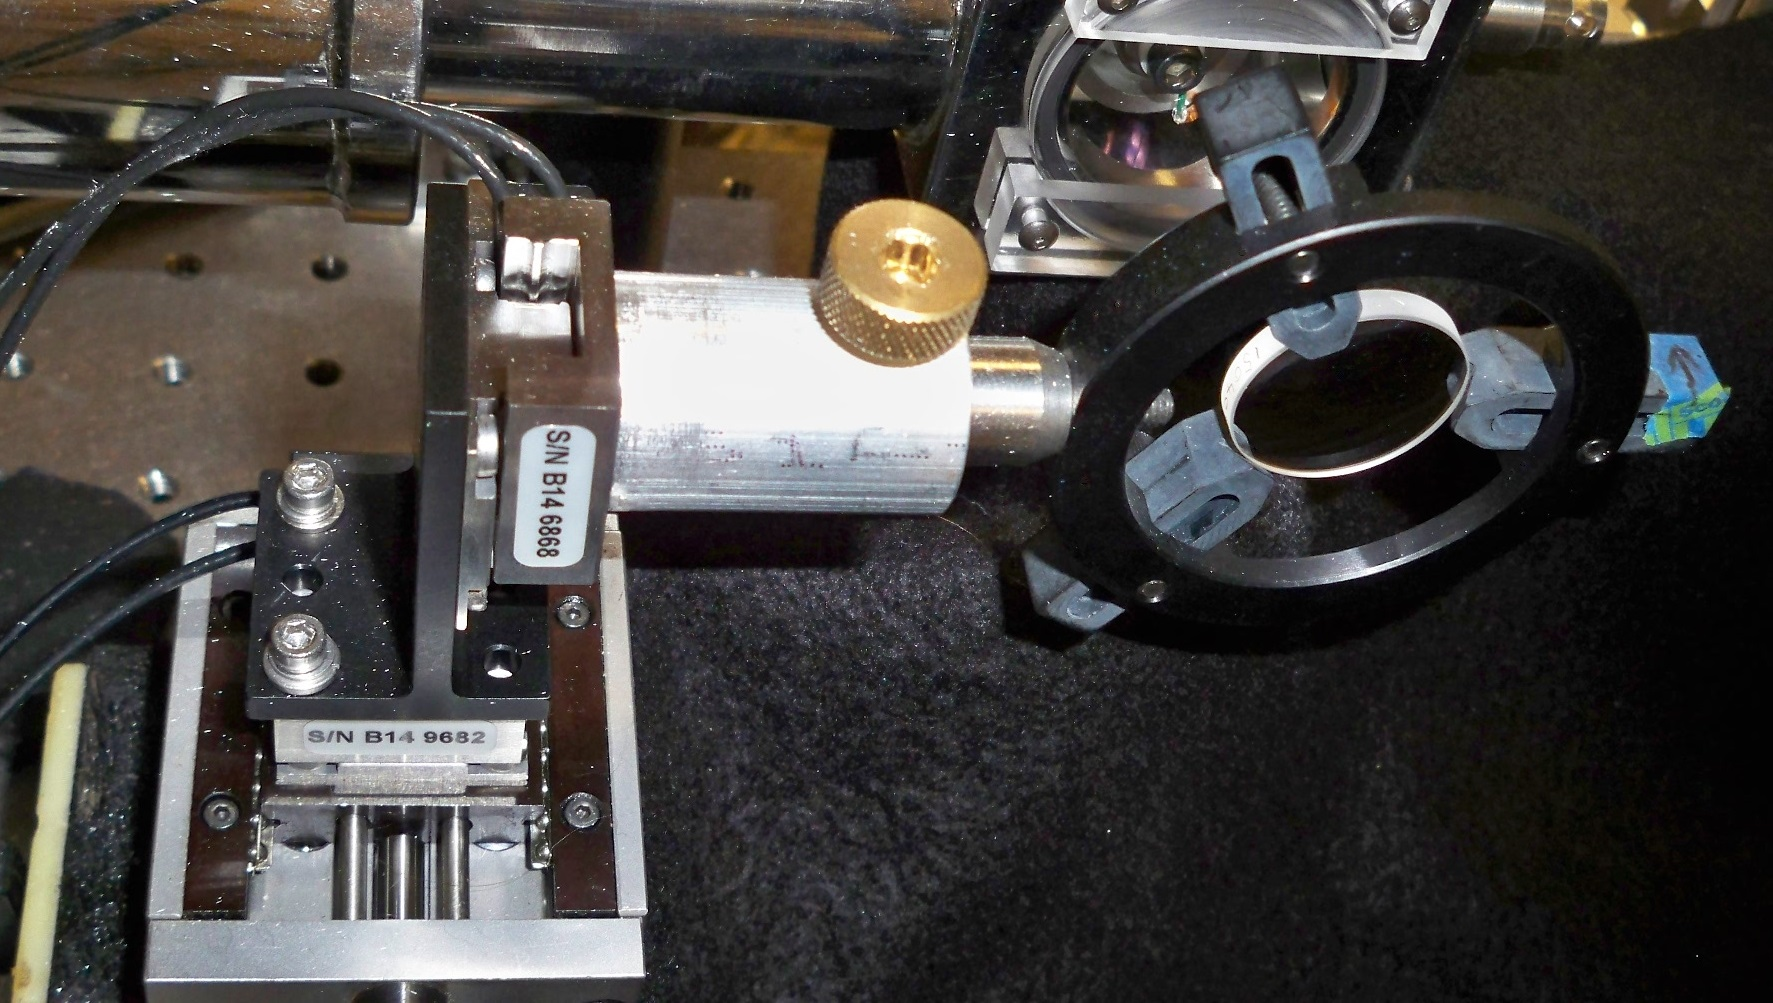
\includegraphics[width=.5\textwidth]{figures/stages_2.JPG}
                \caption{Asphere laser focusing lens mounted to motorized Newport translation stages for laser scanning.}
\label{fig:laserStages}
\end{figure}

\chapter{Results}

Studies of several emission peaks of neutral Ba in SXe are discussed in \ref{sec:fluorescence}.  Bleaching of these peaks is discussed in detail in \ref{sec:bleaching}.  Imaging of Ba fluorescence in a focused laser region is discussed in \ref{imaging}, with the ultimate achievement of imaging at the single atom level using the 619-nm fluorescence peak.  Candidate fluorescence peaks of Ba\textsuperscript{+} in SXe are reported in \ref{sec:BaPlus}.

\section{Fluorescence of Ba in SXe}
\label{sec:fluorescence}

Deposits of Ba in SXe absorb primarily between 540~nm and 570~nm \cite{Mong2015,Brian,Shon}.  An absorption spectrum, obtained by observing absorption of white light by a large Ba deposit at 11~K, is shown in Fig. \ref{fig:BaAbs}, along with an example emission spectrum.  Significant broadening, as well as a 4-nm redshift  of the central peak, occur relative to the vacuum absorption value of 553.5~nm.  Several red-shifted emission peaks are observed and attributed to Ba atoms occupying different matrix sites in the SXe.

\begin{figure} %[H]
        \centering
                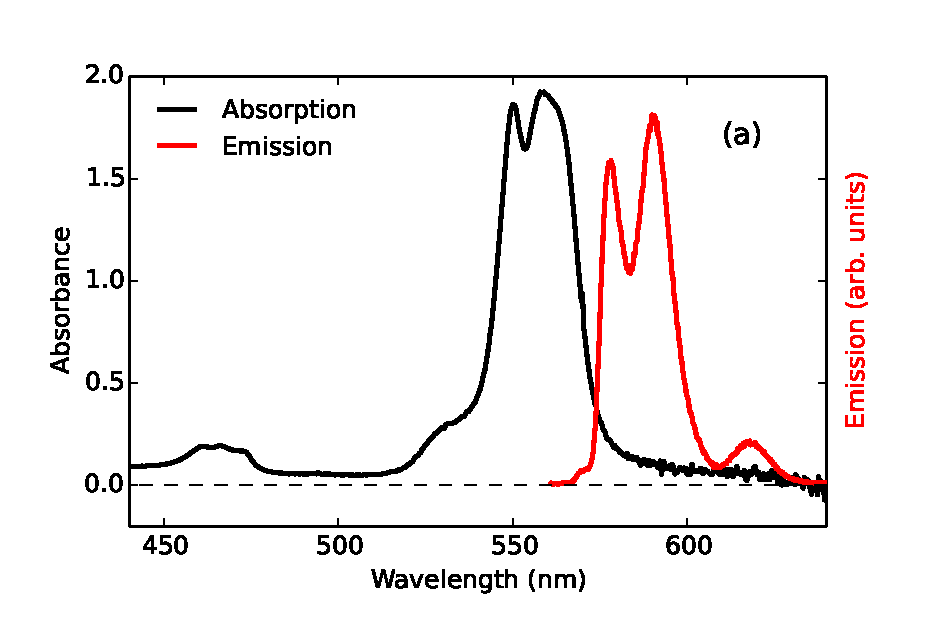
\includegraphics[width=.7\textwidth]{figures/BaAbs_fromBaSpec.eps}
                \caption{\color{red}Get rid of the (a).  Probably need to just edit screenshot with paint.  \cite{Mong2015}}
\label{fig:BaAbs}
\end{figure}

excitspec of 50~K [fig of all, including r110 of 619]... and 10~K?  representative spectra showing all the different peaks

leak rate dependence?

\subsection{Identifying Peaks as Ba in SXe}
\label{subsec:peakIdentify}

\emph{\color{gray}This section was claimed in Ba getter section of Chapter 3 to talk about getter use in identifying 619.}

\subsection{Temperature/annealing}

\section{Bleaching}
\label{sec:bleaching}

({\color{red}do a correction on p-meter sensitive area and on p-meter quantum efficiency, and also a spherical aberation correction for power, though that may not matter for the defocused studies.})

590 etc, model fit (see results intro paragraph)

\begin{figure} %[H]
        \centering
                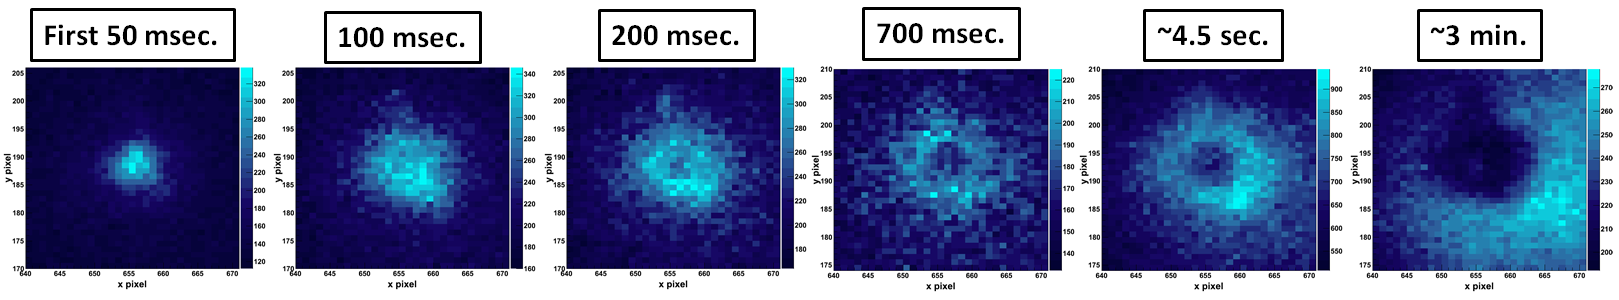
\includegraphics[width=.9\textwidth]{figures/hole_bleach_590.png}
                \caption{}
\label{fig:testfig}
\end{figure}

619, with the changes in time and I

\section{Imaging}
\label{imaging}

\subsection{Imaging 577- and 591-nm peaks}

\subsection{Imaging 619-nm peak}

\begin{figure} %[H]
        \centering
                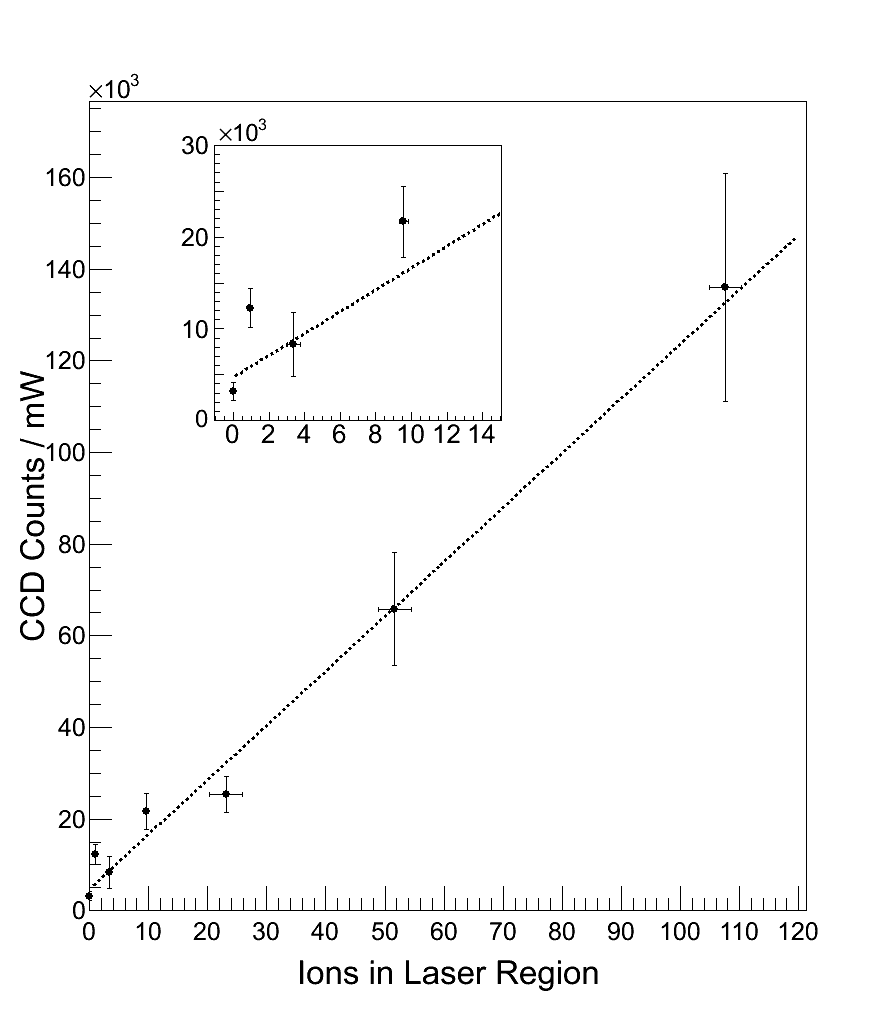
\includegraphics[width=.7\textwidth]{figures/fitgrouped_20150807_20150916_inset.png}
                \caption{Combined 2015-08-07 and 2015-09-16 with statistical errors.  \emph{\color{gray}Move y-axis title over.}}
\label{fig:lin}
\end{figure}

\section{Candidate Ba\textsuperscript{+} Lines}
\label{sec:BaPlus}
\chapter{Conclusions}

The achievement of single-atom-level imaging of Ba atoms in SXe is significant progress toward the ability to tag barium daughters in the nEXO LXe TPC.  Improved studies of the spectroscopy of Ba in SXe have been presented and utilized in reaching this level of sensitivity with the 619-nm fluorescence, as well as in imaging the 577- and 591-nm fluorescence for deposits down to $\leq$ around $10^{3}$ atoms.  Blue excitation of Ba\textsuperscript{+} deposits in SXe has revealed several newly reported emission peaks which are candidates for matrix-isolated Ba\textsuperscript{+} ions.

%neutralized Ba\textsuperscript{+} deposits in SXe have been presented.  Of particular interest was temperature and annealing effects, as well as bleaching effects of the 577-, 591-, and 619-nm fluorescence peaks.  Fluorescence was maximal in deposits made around 50~K and observed at 11~K.  The 577- and 591-nm peaks experience similarly rapid bleaching.  A model applied to bleaching data of the 591-nm peak demonstrated agreement with optical pumping rates of Ba in vacuum near the beginning of the bleaching process, with subsequent deviation.  The 619-nm peak experiences much lower bleaching rates.

%Understanding of these effects aided in the design of imaging experiments.  Imaging of Ba atoms in SXe in a focused laser region was demonstrated down to the $\leq 10^{3}$-atom level using the 577- and 591-nm peaks, and down to the single-atom level using the low-bleaching 619-nm peak.

\section{Future Work}
\label{sec:future}

The next major demonstration will be imaging separate Ba atoms in SXe in scanned images.  As indicated in Sec. \ref{sec:scanning}, overcoming the challenge of variable surface background emission is the first priority.  Studies of fluorescence lifetimes of the 619-nm signal vs. the background using a pulsed laser and a photo-multiplier tube for fast detection will be explored, in order to determine whether a photon-sorting technique may remove background.  The atom counting inherent in scanned images will provide the first measurement of the percentage of deposited Ba\textsuperscript{+} ions visible via the 619-nm fluorescence.

Exploration of re-pumping wavelengths for the 577- and 591-nm peaks, as well as the 570- and 601-nm peaks, will be done using tunable lasers in the infrared.  The ability to count atoms emitting with these different wavelengths would be very valuable.  It is not yet known how deposits made by freezing on a probe in LXe will look.  The ability to count ions will be pursued by continuing study of the candidate Ba\textsuperscript{+} emission peaks with blue excitation.

Final demonstrations of Ba tagging in SXe will be done by grabbing out of LXe on cold probes.  Construction of an apparatus is occurring simultaneously in Fairbank's laboratory by Adam Craycraft, where cold probe can be lowered into a LXe cell.  Ba\textsuperscript{+} will be produced by laser ablation of Ba metal and drifted into the LXe and onto the cold probe by electrodes.  [raising to pumput cuz of T dependence ......]
Talk about Adam's work, show pics and stuff.

%\backmatter %...this doesn't seem to do anything

\appendix %this switches to apppendix mode.  Now any new chapters will be appendices instead of chapters.

\chapter{Supplementary Material} %this will be displayed as an appendix, not a chapter.  Appendices are at the same level in the hierarchy as chapters.

make these also into separate files plz

\section{Some Sample Material}

Did the name for the written material come before the name of the organ? Here~\cite{infodim} is a citation in an appendix.

\chapter{Another Supplement}

% still missing some, like backmatter (what is that?), and bibliography:

% <same preamble as we have here>
% \begin{document}
% \frontmatter
% \begin{abstract}

\begin{center}\textsc{Imaging Single Barium Atoms in Solid Xenon for Barium Tagging in the nEXO Neutrinoless Double Beta Decay Experiment}\end{center}

\vspace{6mm}

The nEXO experiment will search for neutrinoless double beta decay of the isotope \textsuperscript{136}Xe in a ton-scale liquid xenon time projection chamber, in order to probe the Majorana nature of neutrinos. Detecting the daughter \textsuperscript{136}Ba of double beta decay events, called barium tagging, is a technique under investigation which would provide a veto for a background-free measurement. This would involve detecting a single barium ion from within a macroscopic volume of liquid xenon. One proposed barium tagging method is to trap the barium ion in solid xenon at the end of a cold probe, and then detect it by its fluorescence in the solid xenon.  In this thesis, new studies on the spectroscopy of deposits of Ba and Ba\textsuperscript{+} in solid xenon are presented.  Imaging of barium atoms in solid xenon is demonstrated with sensitivity down to the single atom level.  Achievement of this level of sensitivity is a major step toward barium tagging by this method.

%in the search for this decay
\end{abstract}
% \begin{acknowledgements}
Bill, Chris, Adam, Shon, Cesar, Brian, Kendy.

If you want the Leif thing, uncomment it in csuthesis.cls.  It says something like "this dissertation is typeset in ... designed by Leif Anderson.
\end{acknowledgements}
% \maketitle
% \mainmatter
% \input{ch1intro}
% \input{anotherchapter}
% <etc>
% \backmatter
% \bibliographystyle{ieeetr}
% \bibliography{thebib}
% \appendix
% \input{thatappendix}
% \end{document}

\end{document}